% Copyright 2004 by Till Tantau <tantau@users.sourceforge.net>.
%
% In principle, this file can be redistributed and/or modified under
% the terms of the GNU Public License, version 2.
%
% However, this file is supposed to be a template to be modified
% for your own needs. For this reason, if you use this file as a
% template and not specifically distribute it as part of a another
% package/program, I grant the extra permission to freely copy and
% modify this file as you see fit and even to delete this copyright
% notice. 

\documentclass[mathserif, xcolor=table]{beamer}
\usepackage{url}
\usepackage{hyperref}
\usepackage{caption}
\usepackage[round]{natbib}
\usepackage{graphicx}
\usepackage{subcaption}
\usepackage{multicol}
\usepackage{multirow}
\usepackage{booktabs}
\usepackage{dcolumn}
\usepackage{tikz}
\usetikzlibrary{graphs,decorations.pathreplacing}

\setbeamertemplate{caption}[numbered]

% There are many different themes available for Beamer. A comprehensive
% list with examples is given here:
% http://deic.uab.es/~iblanes/beamer_gallery/index_by_theme.html
% You can uncomment the themes below if you would like to use a different
% one:
\usetheme{AnnArbor}
%\usetheme{Antibes}
%\usetheme{Bergen}
%\usetheme{Berkeley}
%\usetheme{Berlin}
%\usetheme{Boadilla}
%\usetheme{boxes}
%\usetheme{CambridgeUS}
%\usetheme{Copenhagen}
%\usetheme{Darmstadt}
%\usetheme{default}
%\usetheme{Frankfurt}
%\usetheme{Goettingen}
%\usetheme{Hannover}
%\usetheme{Ilmenau}
%\usetheme{JuanLesPins}
%\usetheme{Luebeck}
%\usetheme{Madrid}
%\usetheme{Malmoe}
%\usetheme{Marburg}
%\usetheme{Montpellier}
%\usetheme{PaloAlto}
%\usetheme{Pittsburgh}
%\usetheme{Rochester}
%\usetheme{Singapore}
%\usetheme{Szeged}
%\usetheme{Warsaw}
%\useoutertheme{infolines}
%\useinnertheme{rectangles}
\usecolortheme{crane}
% https://en.wikibooks.org/wiki/LaTeX/Presentations

%\definecolor{UTDOrange}{RGB}{223,117,0} 
%\definecolor{UTDGreen}{RGB}{18,71,52}

%\setbeamercolor{palette primary}{bg=UTDOrange,fg=white}
%\setbeamercolor{palette secondary}{bg=UTDOrange,fg=white}
%\setbeamercolor{palette tertiary}{bg=UTDOrange,fg=white}
%\setbeamercolor{palette quaternary}{bg=UTDOrange,fg=white}
%\setbeamercolor{section in toc}{fg=black} % TOC sections

%\setbeamercolor{title}{fg=black, bg=UTDOrange}
%\setbeamercolor{titlelike}{fg=black, bg=UTDOrange}

% Override palette coloring with secondary
%\setbeamercolor{subsection in head/foot}{bg=UTDGreen,fg=white}

\title{Value Of Local Showrooms To Online Competitors}

% A subtitle is optional and this may be deleted
\subtitle{Paper Replication with R}

\author{\textbf{Author}: Jayarajan Samuel, Zhiqiang (Eric) Zheng, Ying Xie \\ 
{\footnotesize \textbf{Group Members}: Luoying Chen, Beyza Celik, Duc Vu, Yihong Liu }}

% - Give the names in the same order as the appear in the paper.
% - Use the \inst{?} command only if the authors have different
%   affiliation.

\institute[] % (optional, but mostly needed)
{  
%  \inst{1}%
%  Marketing \\ London Business School
%  
%  \inst{2}%
%  Marketing \\ Massachusetts Institute of Technology
%  
%  \inst{3}%
%  Naveen Jindal School of Management \\ University of Texas at Dallas \\ \url{https://liu-yihong.github.io/}
}
% - Use the \inst command only if there are several affiliations.
% - Keep it simple, no one is interested in your street address.

\date{\today}
% - Either use conference name or its abbreviation.
% - Not really informative to the audience, more for people (including
%   yourself) who are reading the slides online

\subject{Management Science}
% This is only inserted into the PDF information catalog. Can be left
% out. 

% If you have a file called "university-logo-filename.xxx", where xxx
% is a graphic format that can be processed by latex or pdflatex,
% resp., then you can add a logo as follows:

\pgfdeclareimage[height=0.9cm]{university-logo}{header-JSOM-Black2.png}
\logo{\pgfuseimage{university-logo}}

% Delete this, if you do not want the table of contents to pop up at
% the beginning of each subsection:

%\AtBeginSubsection[]
%{
%  \begin{frame}<beamer>{Outline}
%    \tableofcontents[currentsection,currentsubsection]
%  \end{frame}
%}

%gets rid of bottom navigation bars
\setbeamertemplate{footline}[page number]{}

%gets rid of navigation symbols
\setbeamertemplate{navigation symbols}{}

% Let's get started
\begin{document}

\begin{frame}
  \titlepage
\end{frame}

\begin{frame}[allowframebreaks]{Outline}
  \tableofcontents
  % You might wish to add the option [pausesections]
\end{frame}

\section{Background}
\begin{frame}[allowframebreaks]{Background}
	\begin{itemize}
		\item Online Shopping vs Offline
		\begin{multicols}{2}
			\begin{itemize}
				\item Online Info Hub
				\begin{enumerate}
					\item Usually lower price
					\item Various types
					\item Less time
				\end{enumerate}
				\item Offline Showroom
				\begin{enumerate}
					\item Physically experienced
					\item Real-time assistance
					\item Instant gratification
				\end{enumerate}
			\end{itemize}
		\end{multicols}
		\item Customer interacts between online and offline
	\end{itemize}
	\framebreak
	\begin{figure}[h]
		\centering
		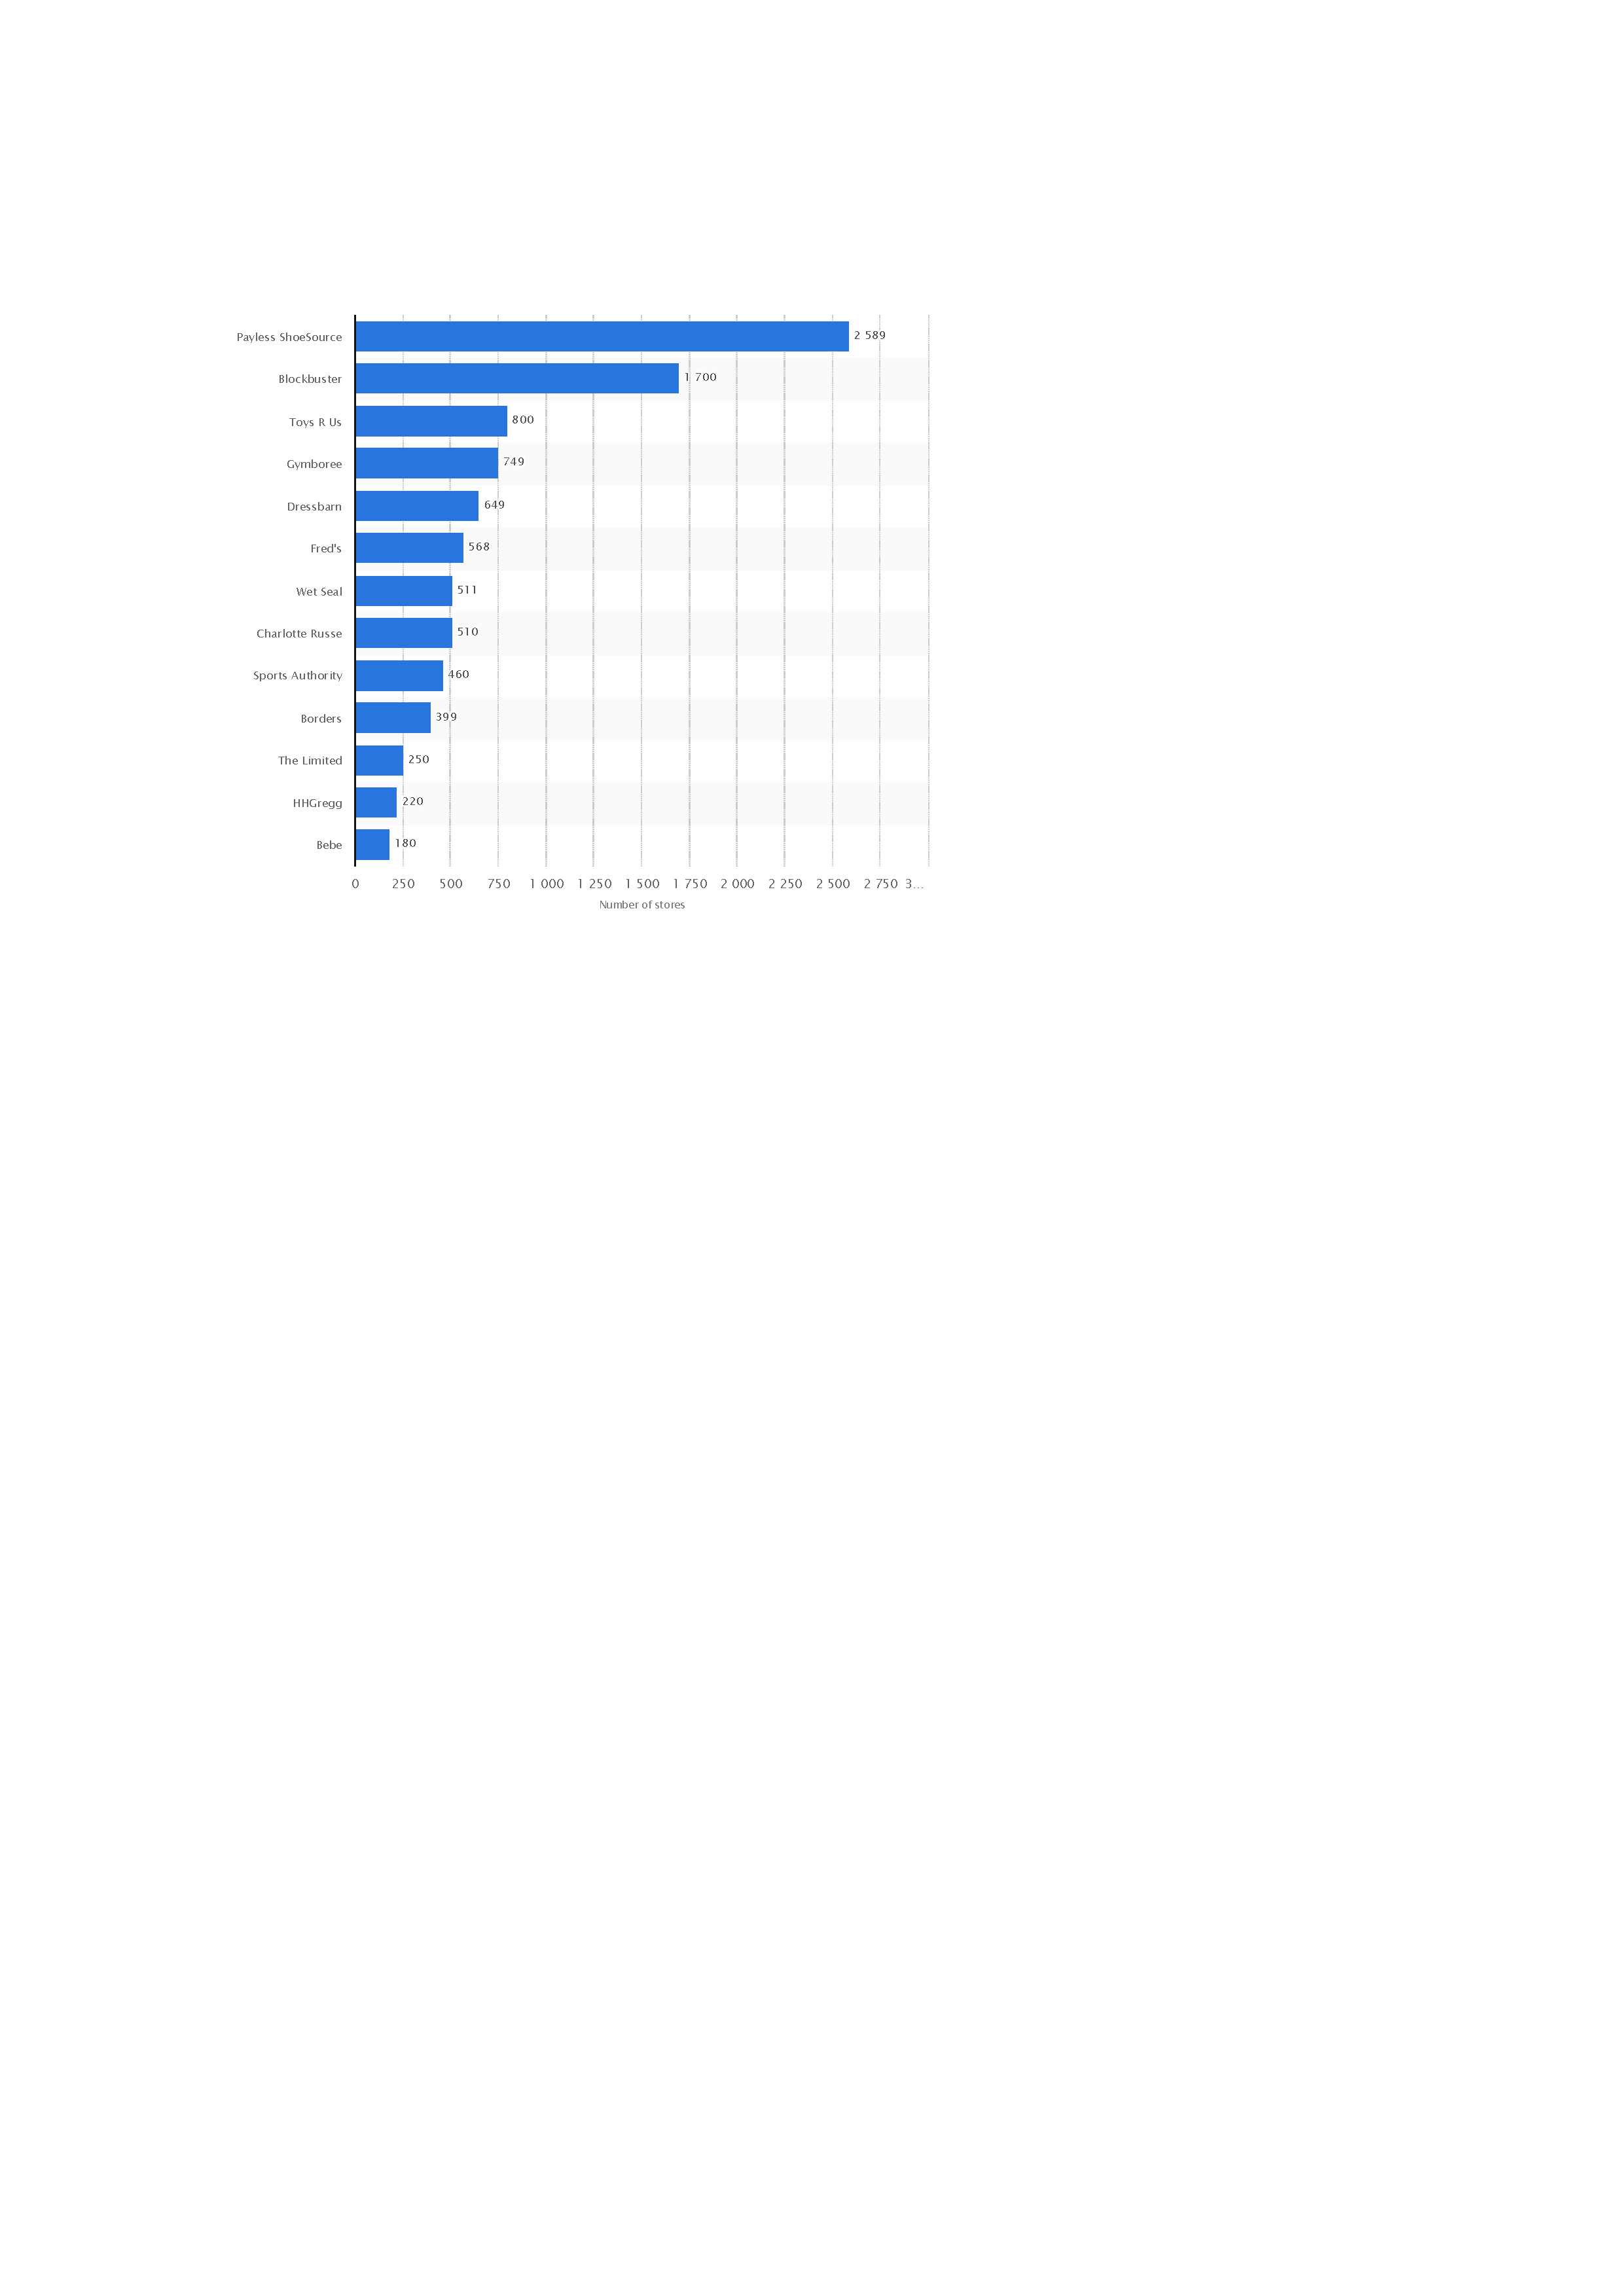
\includegraphics[scale=0.3]{pic/retail_closure.pdf}
		\caption{Num Of Store Closures by Selected Retailers in US From 2010 to 2020 \footnote{\href{https://www.statista.com/statistics/1092243/number-of-stores-closures-by-selected-retailers-us/}{source link: statista.com}}}
	\end{figure}
	\begin{itemize}
		\item Values of offline store closures for online retailers?
	\end{itemize}
\end{frame}

\section{Research Questions}
\begin{frame}{Research Questions}
	\begin{enumerate}
		\item How would a retailer closing a physical store impact
		\begin{itemize}
			\item its customers’ shopping searching behaviors, 
			\item their resultant purchasing behaviors
		\end{itemize}
	 with an online competitor?
	\end{enumerate}
\end{frame}

\section{Data}
\begin{frame}{Data Description}
	\begin{itemize}
		\item Natural Experiment: Circuit City closed 155 local stores (physical showroom providers) due to severe competitions (exogenous event) on Nov, 2008
		\item Data Scheme: individual customer click-stream dataset (search and purchase) during each month of 2008 and 2009
		\begin{multicols}{3}
			\begin{itemize}
				\item time stamp
				\item visited domain 
				\item referring domain
				\item \# of pages
				\item Duration
				\item Purchase Flag
				\item Paid Amount
				\item Zip Code
				\item Demographics
			\end{itemize}
		\end{multicols}
		\item Focused Online Retailer: Amazon (pure) and Bestbuy (multi)
		\item Treatment: Residents in 155 Zip codes / 5-miles radius of 155
		\item Control: Residents who never had CC stores within 5 miles 
	\end{itemize}
\end{frame}

\begin{frame}{Data Process}
	\begin{itemize}
		\item Referring Domain Filter: blank or search engine
		\item Target Domain Filter: amazon, staples, dell, walmart, bestbuy
		\item Product Categories Filter: only types sold at CC
		\item Variables Construction:
		\begin{itemize}
			\begin{multicols}{2}
				\item \texttt{CCStorePresent}
				\item \textsf{AfterStoreClosing}
				\item \textsf{BBStorePresent}
				\item \textsf{NoReferringDomain}
				\item \textsf{ReferringDomainIsSearchEngine}
				\item \textsf{Dependent Variables}
			\end{multicols}
		\end{itemize}
		\item Panel Data Aggregation
		\begin{itemize}
			\item Group by Zip Code, Month-Year, Target Domain
			\item Calculate Dependent Variables
			\item Unbalanced Data Imputation
		\end{itemize}
	\end{itemize}
\end{frame}

\section{Results Replication}

\subsection{Effects on Online Sales}
\begin{frame}[allowframebreaks]{Effects on Online Sales}
	To examine whether a competing online retailer benefits from the presence of a local showroom, we run the following regressions for Amazon and BestBuy
	\begin{equation}
		\begin{aligned}
			& \log\left( \texttt{TotalMonthlySales} + 1\right)_{i,t} \\ &= \mu_{i} + \tau_{t} 
			\\ &+ \beta_1 \ \texttt{CCStorePresent}_i \times \texttt{AfterStoreClosing}_t 
			\\ &+ \beta_2 \ \texttt{CCStorePresent}_i \times \texttt{AfterStoreClosing}_t \times \texttt{BBStorePresent}_i \\ & + \epsilon_{i,t}
		\end{aligned}
	\end{equation}
	\framebreak
	\begin{table}[!h] \centering 
		\caption{Results of the Sales Effect (All Product Categories)} 
		\label{tab:table4} 
		\resizebox{\columnwidth}{!}{
			\begin{tabular}{@{\extracolsep{1pt}}lD{.}{.}{-3} D{.}{.}{-3} D{.}{.}{-3} D{.}{.}{-3} } 
				\\[-1.8ex]\hline 
				\hline \\[-1.8ex] 
				% & \multicolumn{4}{c}{\textit{Dependent variable:}} \\ 
				% \cline{2-5} 
				% \\[-1.8ex] 
				& \multicolumn{4}{c}{log(TotalMonthlySales + 1)} \\ 
				& \multicolumn{1}{c}{Amazon-0 Mile} & \multicolumn{1}{c}{Amazon-5 Miles} & \multicolumn{1}{c}{BestBuy-0 Mile} & \multicolumn{1}{c}{BestBuy-5 Miles} \\ 
				\\[-1.8ex] & \multicolumn{1}{c}{(1)} & \multicolumn{1}{c}{(2)} & \multicolumn{1}{c}{(3)} & \multicolumn{1}{c}{(4)}\\ 
				\hline \\[-1.8ex] 
				$\beta_1$ & 0.014 & -0.005 & -0.002 & -0.002 \\ 
				& (0.015) & (0.008) & (0.033) & (0.008) \\ 
				$\beta_2$ & -0.033 & 0.003 & 0.009 & 0.002 \\ 
				& (0.022) & (0.010) & (0.036) & (0.010) \\ 
				\hline \\[-1.8ex] 
				Observations & \multicolumn{1}{c}{68,472} & \multicolumn{1}{c}{75,096} & \multicolumn{1}{c}{14,664} & \multicolumn{1}{c}{16,848} \\ 
				R$^{2}$ & \multicolumn{1}{c}{0.00003} & \multicolumn{1}{c}{0.00001} & \multicolumn{1}{c}{0.00002} & \multicolumn{1}{c}{0.00000} \\ 
				Adjusted R$^{2}$ & \multicolumn{1}{c}{-0.044} & \multicolumn{1}{c}{-0.044} & \multicolumn{1}{c}{-0.045} & \multicolumn{1}{c}{-0.045} \\ 
				F Statistic & \multicolumn{1}{c}{1.091 (df = 2; 65594)} & \multicolumn{1}{c}{0.278 (df = 2; 71942)} & \multicolumn{1}{c}{0.154 (df = 2; 14028)} & \multicolumn{1}{c}{0.035 (df = 2; 16121)} \\  
				\hline 
				\hline \\[-1.8ex] 
				\textit{Note:}  & \multicolumn{4}{r}{$^{*}$p$<$0.1; $^{**}$p$<$0.05; $^{***}$p$<$0.01} \\ 
			\end{tabular} 
		}
	\end{table}
\end{frame}

\subsection{Effects on Online Search Behavior}
\begin{frame}[allowframebreaks]{Effects on Online Search Behavior}
	To measure the impact of the exit of local showrooms on consumer online search intensity and the moderating effect of Best Buy Stores as an alternative local showroom, we run the following regressions
	\begin{equation}
		\begin{aligned}
			& \log\left( \texttt{PagesPerDollar} + 1,\ \texttt{MinsPerDollar} + 1\right)_{i,t} \\ &= \mu_{i} + \tau_{t} 
			\\ &+ \beta_1 \ \texttt{CCStorePresent}_i \times \texttt{AfterStoreClosing}_t 
			\\ &+ \beta_2 \ \texttt{CCStorePresent}_i \times \texttt{AfterStoreClosing}_t \times \texttt{BBStorePresent}_i \\ & + \epsilon_{i,t}
		\end{aligned}
	\end{equation}
	\framebreak
	\begin{table}[!htbp] \centering 
		\caption{Results of the Search Effect (All Product Categories)} 
		\label{tab:table5} 
		\resizebox{\columnwidth}{!}{
			\begin{tabular}{@{\extracolsep{1pt}}lD{.}{.}{-3} D{.}{.}{-3} D{.}{.}{-3} D{.}{.}{-3} D{.}{.}{-3} D{.}{.}{-3} D{.}{.}{-3} D{.}{.}{-3} } 
				\\[-1.8ex]\hline 
				\hline \\[-1.8ex] 
				%& \multicolumn{8}{c}{\textit{Dependent variable:}} \\ 
				%\cline{2-9} 
				%\\[-1.8ex] 
				& \multicolumn{4}{c}{log(PagesPerDollar + 1)} & \multicolumn{4}{c}{log(MinsPerDollar + 1)} \\ 
				& \multicolumn{1}{c}{Amazon-0 Mile} & \multicolumn{1}{c}{Amazon-5 Miles} & \multicolumn{1}{c}{BestBuy-0 Mile} & \multicolumn{1}{c}{BestBuy-5 Miles} & \multicolumn{1}{c}{Amazon-0 Mile} & \multicolumn{1}{c}{Amazon-5 Miles} & \multicolumn{1}{c}{BestBuy-0 Mile} & \multicolumn{1}{c}{BestBuy-5 Miles} \\ 
				\\[-1.8ex] & \multicolumn{1}{c}{(1)} & \multicolumn{1}{c}{(2)} & \multicolumn{1}{c}{(3)} & \multicolumn{1}{c}{(4)} & \multicolumn{1}{c}{(5)} & \multicolumn{1}{c}{(6)} & \multicolumn{1}{c}{(7)} & \multicolumn{1}{c}{(8)}\\ 
				\hline \\[-1.8ex] 
				$\beta_1$ & 0.003 & -0.019^{***} & 0.001 & 0.002 & 0.004 & -0.021^{***} & 0.001 & 0.003 \\ 
				& (0.012) & (0.007) & (0.016) & (0.004) & (0.012) & (0.007) & (0.013) & (0.003) \\ 
				$\beta_2$ & -0.068^{***} & 0.018^{**} & 0.003 & -0.001 & -0.057^{***} & 0.022^{***} & 0.0004 & -0.002 \\ 
				& (0.018) & (0.009) & (0.018) & (0.005) & (0.017) & (0.008) & (0.014) & (0.004) \\ 
				\hline \\[-1.8ex] 
				Observations & \multicolumn{1}{c}{68,472} & \multicolumn{1}{c}{75,096} & \multicolumn{1}{c}{14,664} & \multicolumn{1}{c}{16,848} & \multicolumn{1}{c}{68,472} & \multicolumn{1}{c}{75,096} & \multicolumn{1}{c}{14,664} & \multicolumn{1}{c}{16,848} \\ 
				R$^{2}$ & \multicolumn{1}{c}{0.0004} & \multicolumn{1}{c}{0.0001} & \multicolumn{1}{c}{0.00003} & \multicolumn{1}{c}{0.00004} & \multicolumn{1}{c}{0.0003} & \multicolumn{1}{c}{0.0001} & \multicolumn{1}{c}{0.00001} & \multicolumn{1}{c}{0.0001} \\ 
				Adjusted R$^{2}$ & \multicolumn{1}{c}{-0.043} & \multicolumn{1}{c}{-0.044} & \multicolumn{1}{c}{-0.045} & \multicolumn{1}{c}{-0.045} & \multicolumn{1}{c}{-0.044} & \multicolumn{1}{c}{-0.044} & \multicolumn{1}{c}{-0.045} & \multicolumn{1}{c}{-0.045} \\ 
				F Statistic & \multicolumn{1}{c}{12.530$^{***}$ (df = 2; 65594)} & \multicolumn{1}{c}{3.985$^{**}$ (df = 2; 71942)} & \multicolumn{1}{c}{0.202 (df = 2; 14028)} & \multicolumn{1}{c}{0.337 (df = 2; 16121)} & \multicolumn{1}{c}{8.867$^{***}$ (df = 2; 65594)} & \multicolumn{1}{c}{5.187$^{***}$ (df = 2; 71942)} & \multicolumn{1}{c}{0.046 (df = 2; 14028)} & \multicolumn{1}{c}{0.451 (df = 2; 16121)} \\ 
				\hline 
				\hline \\[-1.8ex] 
				\textit{Note:}  & \multicolumn{8}{r}{$^{*}$p$<$0.1; $^{**}$p$<$0.05; $^{***}$p$<$0.01} \\ 
			\end{tabular} 
		}
	\end{table}
\end{frame}

\subsection{Effects on Online Sales vs Prod Types}
\begin{frame}[allowframebreaks]{Effects on Online Sales vs Prod Types}
	We then test whether the show-rooming effect upon online sales is stronger for experience goods.
	\begin{table}[!h] \centering 
		\caption{Results of the Sales Effect: Experience and Search Products} 
		\label{tab:table6} 
		\resizebox{\columnwidth}{!}{
			\begin{tabular}{@{\extracolsep{1pt}}lD{.}{.}{-3} D{.}{.}{-3} D{.}{.}{-3} D{.}{.}{-3} D{.}{.}{-3} D{.}{.}{-3} D{.}{.}{-3} D{.}{.}{-3} } 
				\\[-1.8ex]\hline 
				\hline \\[-1.8ex] 
				%& \multicolumn{8}{c}{\textit{Dependent variable:}} \\ 
				%\cline{2-9} 
				%\\[-1.8ex] 
				& \multicolumn{8}{c}{log(TotalMonthlySales + 1)} \\ 
				& \multicolumn{1}{c}{Amazon-0 Mile-Exp} & \multicolumn{1}{c}{Amazon-5 Miles-Exp} & \multicolumn{1}{c}{Amazon-0 Mile-Search} & \multicolumn{1}{c}{Amazon-5 Miles-Search} & \multicolumn{1}{c}{BestBuy-0 Mile-Exp} & \multicolumn{1}{c}{BestBuy-5 Miles-Exp} & \multicolumn{1}{c}{BestBuy-0 Mile-Exp} & \multicolumn{1}{c}{BestBuy-5 Miles-Search} \\ 
				\\[-1.8ex] & \multicolumn{1}{c}{(1)} & \multicolumn{1}{c}{(2)} & \multicolumn{1}{c}{(3)} & \multicolumn{1}{c}{(4)} & \multicolumn{1}{c}{(5)} & \multicolumn{1}{c}{(6)} & \multicolumn{1}{c}{(7)} & \multicolumn{1}{c}{(8)}\\ 
				\hline \\[-1.8ex] 
				$\beta_1$ & 0.005 & -0.007 & 0.005 & -0.008 & -0.011 & -0.009 & -0.001 & -0.010 \\ 
				& (0.017) & (0.010) & (0.013) & (0.006) & (0.009) & (0.007) & (0.023) & (0.008) \\ 
				$\beta_2$ & -0.043^{*} & 0.009 & -0.002 & 0.009 &  & 0.013 & 0.000 & 0.009 \\ 
				& (0.024) & (0.012) & (0.018) & (0.008) &  & (0.008) & (0.028) & (0.010) \\ 
				\hline \\[-1.8ex] 
				Observations & \multicolumn{1}{c}{32,112} & \multicolumn{1}{c}{35,568} & \multicolumn{1}{c}{52,392} & \multicolumn{1}{c}{57,648} & \multicolumn{1}{c}{10,224} & \multicolumn{1}{c}{11,712} & \multicolumn{1}{c}{5,664} & \multicolumn{1}{c}{6,600} \\ 
				R$^{2}$ & \multicolumn{1}{c}{0.0002} & \multicolumn{1}{c}{0.00002} & \multicolumn{1}{c}{0.00000} & \multicolumn{1}{c}{0.00003} & \multicolumn{1}{c}{0.0001} & \multicolumn{1}{c}{0.0002} & \multicolumn{1}{c}{0.00000} & \multicolumn{1}{c}{0.0002} \\ 
				Adjusted R$^{2}$ & \multicolumn{1}{c}{-0.044} & \multicolumn{1}{c}{-0.044} & \multicolumn{1}{c}{-0.044} & \multicolumn{1}{c}{-0.044} & \multicolumn{1}{c}{-0.046} & \multicolumn{1}{c}{-0.045} & \multicolumn{1}{c}{-0.048} & \multicolumn{1}{c}{-0.047} \\ 
				F Statistic & \multicolumn{1}{c}{2.775$^{*}$ (df = 2; 30749)} & \multicolumn{1}{c}{0.318 (df = 2; 34061)} & \multicolumn{1}{c}{0.101 (df = 2; 50184)} & \multicolumn{1}{c}{0.774 (df = 2; 55221)} & \multicolumn{1}{c}{1.377 (df = 1; 9774)} & \multicolumn{1}{c}{1.297 (df = 2; 11199)} & \multicolumn{1}{c}{0.004 (df = 2; 5403)} & \multicolumn{1}{c}{0.746 (df = 2; 6300)} \\ 
				\hline 
				\hline \\[-1.8ex] 
				\textit{Note:}  & \multicolumn{8}{r}{$^{*}$p$<$0.1; $^{**}$p$<$0.05; $^{***}$p$<$0.01} \\ 
		\end{tabular} }
	\end{table}
\end{frame}

\subsection{Effects on Online Search Behavior vs Prod Types}
\begin{frame}[allowframebreaks]{Effects on Online Search Behavior vs Prod Types}
	We want to test whether the show-rooming effect is stronger for experience goods
	\begin{table}[!h] \centering 
		\caption{Results of the Online Search Effect: Experience Products} 
		\label{tab:table7} 
		\resizebox{\columnwidth}{!}{
			\begin{tabular}{@{\extracolsep{1pt}}lD{.}{.}{-3} D{.}{.}{-3} D{.}{.}{-3} D{.}{.}{-3} D{.}{.}{-3} D{.}{.}{-3} D{.}{.}{-3} D{.}{.}{-3} } 
				\\[-1.8ex]\hline 
				\hline \\[-1.8ex] 
				%& \multicolumn{8}{c}{\textit{Dependent variable:}} \\ 
				%\cline{2-9} 
				%\\[-1.8ex] 
				& \multicolumn{4}{c}{log(PagesPerDollar + 1)} & \multicolumn{4}{c}{log(MinsPerDollar + 1)} \\ 
				& \multicolumn{1}{c}{Amazon-0 Mile} & \multicolumn{1}{c}{Amazon-5 Miles} & \multicolumn{1}{c}{BestBuy-0 Mile} & \multicolumn{1}{c}{BestBuy-5 Miles} & \multicolumn{1}{c}{Amazon-0 Mile} & \multicolumn{1}{c}{Amazon-5 Miles} & \multicolumn{1}{c}{BestBuy-0 Mile} & \multicolumn{1}{c}{BestBuy-5 Miles} \\ 
				\\[-1.8ex] & \multicolumn{1}{c}{(1)} & \multicolumn{1}{c}{(2)} & \multicolumn{1}{c}{(3)} & \multicolumn{1}{c}{(4)} & \multicolumn{1}{c}{(5)} & \multicolumn{1}{c}{(6)} & \multicolumn{1}{c}{(7)} & \multicolumn{1}{c}{(8)}\\ 
				\hline \\[-1.8ex] 
				$\beta_1$ & 0.007 & -0.037^{***} & 0.006^{**} & 0.001 & 0.006 & -0.039^{***} & 0.003 & 0.001 \\ 
				& (0.015) & (0.008) & (0.002) & (0.002) & (0.015) & (0.008) & (0.002) & (0.001) \\ 
				$\beta_2$ & -0.077^{***} & 0.030^{***} &  & -0.0001 & -0.067^{***} & 0.034^{***} &  & -0.001 \\ 
				& (0.020) & (0.010) &  & (0.002) & (0.020) & (0.010) &  & (0.002) \\ 
				\hline \\[-1.8ex] 
				Observations & \multicolumn{1}{c}{32,112} & \multicolumn{1}{c}{35,568} & \multicolumn{1}{c}{10,224} & \multicolumn{1}{c}{11,712} & \multicolumn{1}{c}{32,112} & \multicolumn{1}{c}{35,568} & \multicolumn{1}{c}{10,224} & \multicolumn{1}{c}{11,712} \\ 
				R$^{2}$ & \multicolumn{1}{c}{0.001} & \multicolumn{1}{c}{0.001} & \multicolumn{1}{c}{0.001} & \multicolumn{1}{c}{0.00003} & \multicolumn{1}{c}{0.001} & \multicolumn{1}{c}{0.001} & \multicolumn{1}{c}{0.0003} & \multicolumn{1}{c}{0.0001} \\ 
				Adjusted R$^{2}$ & \multicolumn{1}{c}{-0.043} & \multicolumn{1}{c}{-0.044} & \multicolumn{1}{c}{-0.045} & \multicolumn{1}{c}{-0.046} & \multicolumn{1}{c}{-0.044} & \multicolumn{1}{c}{-0.044} & \multicolumn{1}{c}{-0.046} & \multicolumn{1}{c}{-0.046} \\ 
				F Statistic & \multicolumn{1}{c}{12.857$^{***}$ (df = 2; 30749)} & \multicolumn{1}{c}{10.009$^{***}$ (df = 2; 34061)} & \multicolumn{1}{c}{5.763$^{**}$ (df = 1; 9774)} & \multicolumn{1}{c}{0.143 (df = 2; 11199)} & \multicolumn{1}{c}{10.349$^{***}$ (df = 2; 30749)} & \multicolumn{1}{c}{11.626$^{***}$ (df = 2; 34061)} & \multicolumn{1}{c}{2.508 (df = 1; 9774)} & \multicolumn{1}{c}{0.438 (df = 2; 11199)} \\ 
				\hline 
				\hline \\[-1.8ex] 
				\textit{Note:}  & \multicolumn{8}{r}{$^{*}$p$<$0.1; $^{**}$p$<$0.05; $^{***}$p$<$0.01} \\ 
		\end{tabular} }
	\end{table}
\framebreak
\begin{table}[!h] \centering 
	\caption{Results of the Online Search Effect: Search Products} 
	\label{tab:table8} 
	\resizebox{\columnwidth}{!}{
		\begin{tabular}{@{\extracolsep{1pt}}lD{.}{.}{-3} D{.}{.}{-3} D{.}{.}{-3} D{.}{.}{-3} D{.}{.}{-3} D{.}{.}{-3} D{.}{.}{-3} D{.}{.}{-3} } 
			\\[-1.8ex]\hline 
			\hline \\[-1.8ex] 
			%& \multicolumn{8}{c}{\textit{Dependent variable:}} \\ 
			%\cline{2-9} 
			%\\[-1.8ex] 
			& \multicolumn{4}{c}{log(PagesPerDollar + 1)} & \multicolumn{4}{c}{log(MinsPerDollar + 1)} \\ 
			& \multicolumn{1}{c}{Amazon-0 Mile} & \multicolumn{1}{c}{Amazon-5 Miles} & \multicolumn{1}{c}{BestBuy-0 Mile} & \multicolumn{1}{c}{BestBuy-5 Miles} & \multicolumn{1}{c}{Amazon-0 Mile} & \multicolumn{1}{c}{Amazon-5 Miles} & \multicolumn{1}{c}{BestBuy-0 Mile} & \multicolumn{1}{c}{BestBuy-5 Miles} \\ 
			\\[-1.8ex] & \multicolumn{1}{c}{(1)} & \multicolumn{1}{c}{(2)} & \multicolumn{1}{c}{(3)} & \multicolumn{1}{c}{(4)} & \multicolumn{1}{c}{(5)} & \multicolumn{1}{c}{(6)} & \multicolumn{1}{c}{(7)} & \multicolumn{1}{c}{(8)}\\ 
			\hline \\[-1.8ex] 
			$\beta_1$ & 0.001 & 0.006 & 0.001 & 0.009^{*} & 0.003 & 0.004 & 0.0001 & 0.009^{*} \\ 
			& (0.012) & (0.006) & (0.014) & (0.005) & (0.012) & (0.006) & (0.012) & (0.005) \\ 
			$\beta_2$ & -0.019 & -0.002 & -0.000 & -0.007 & -0.019 & 0.001 & -0.000 & -0.008 \\ 
			& (0.017) & (0.008) & (0.017) & (0.006) & (0.017) & (0.008) & (0.015) & (0.006) \\ 
			\hline \\[-1.8ex] 
			Observations & \multicolumn{1}{c}{52,392} & \multicolumn{1}{c}{57,648} & \multicolumn{1}{c}{5,664} & \multicolumn{1}{c}{6,600} & \multicolumn{1}{c}{52,392} & \multicolumn{1}{c}{57,648} & \multicolumn{1}{c}{5,664} & \multicolumn{1}{c}{6,600} \\ 
			R$^{2}$ & \multicolumn{1}{c}{0.00005} & \multicolumn{1}{c}{0.00002} & \multicolumn{1}{c}{0.00000} & \multicolumn{1}{c}{0.001} & \multicolumn{1}{c}{0.00004} & \multicolumn{1}{c}{0.00003} & \multicolumn{1}{c}{0.00000} & \multicolumn{1}{c}{0.001} \\ 
			Adjusted R$^{2}$ & \multicolumn{1}{c}{-0.044} & \multicolumn{1}{c}{-0.044} & \multicolumn{1}{c}{-0.048} & \multicolumn{1}{c}{-0.047} & \multicolumn{1}{c}{-0.044} & \multicolumn{1}{c}{-0.044} & \multicolumn{1}{c}{-0.048} & \multicolumn{1}{c}{-0.047} \\ 
			F Statistic & \multicolumn{1}{c}{1.138 (df = 2; 50184)} & \multicolumn{1}{c}{0.553 (df = 2; 55221)} & \multicolumn{1}{c}{0.011 (df = 2; 5403)} & \multicolumn{1}{c}{1.590 (df = 2; 6300)} & \multicolumn{1}{c}{0.935 (df = 2; 50184)} & \multicolumn{1}{c}{0.696 (df = 2; 55221)} & \multicolumn{1}{c}{0.0001 (df = 2; 5403)} & \multicolumn{1}{c}{1.927 (df = 2; 6300)} \\ 
			\hline 
			\hline \\[-1.8ex] 
			\textit{Note:}  & \multicolumn{8}{r}{$^{*}$p$<$0.1; $^{**}$p$<$0.05; $^{***}$p$<$0.01} \\ 
	\end{tabular} }
\end{table}
\end{frame}

\subsection{Effects on Referring Domain}

\begin{frame}[allowframebreaks]{Effects on Referring Domain}
	To capture the expected change in the odds ratio of the impact of Circuit City store closures and
	the moderating effect of Best Buy stores as an alternative local showroom, we run the following regressions:
	\begin{equation}
		\begin{aligned}
			& \textrm{Logit}\left( \texttt{ReferringDomainIsSearchEngine}, \texttt{NoReferringDomain} \right)_{i,t} \\ &= \mu_{i} + \tau_{t} 
			\\ &+ \beta_1 \ \texttt{CCStorePresent}_i \times \texttt{AfterStoreClosing}_t 
			\\ &+ \beta_2 \ \texttt{CCStorePresent}_i \times \texttt{AfterStoreClosing}_t \times \texttt{BBStorePresent}_i \\ & + \epsilon_{i,t}
		\end{aligned}
	\end{equation}
	\framebreak
	Table \ref{tab:table9} presents the effect of store closure on referring domain.
	\begin{table}[!h] \centering 
		\caption{Results of Logistic Regression for Referring Domain} 
		\label{tab:table9} 
		\resizebox{\columnwidth}{!}{
			\begin{tabular}{@{\extracolsep{1pt}}lD{.}{.}{-3} D{.}{.}{-3} D{.}{.}{-3} D{.}{.}{-3} } 
				\\[-1.8ex]\hline 
				\hline \\[-1.8ex] 
				% & \multicolumn{4}{c}{\textit{Dependent variable:}} \\ 
				% \cline{2-5} 
				% \\[-1.8ex] 
				& \multicolumn{2}{c}{ReferringDomainIsSearchEngine} & \multicolumn{2}{c}{NoReferringDomain} \\
				& \multicolumn{1}{c}{Amazon-0 Mile} & \multicolumn{1}{c}{BestBuy-0 Mile} & \multicolumn{1}{c}{Amazon-0 Mile} & \multicolumn{1}{c}{BestBuy-0 Mile} \\ 
				\\[-1.8ex] & \multicolumn{1}{c}{(1)} & \multicolumn{1}{c}{(2)} & \multicolumn{1}{c}{(3)} & \multicolumn{1}{c}{(4)}\\ 
				\hline \\[-1.8ex] 
				$\beta_1$ & -0.817^{*} & -15.12^{***} & 0.325 & -0.223 \\ 
				& (0.337)  & (0.611) & (0.346) & (1.259) \\ 
				$\beta_2$ & 0.697 & 14.43^{***} & -0.415 & 0.916 \\ 
				& (0.564) & (0.944) & (0.544) & (1.615) \\ 
				\hline \\[-1.8ex] 
				Observations & \multicolumn{1}{c}{10,791} & \multicolumn{1}{c}{1,225} & \multicolumn{1}{c}{10,791} & \multicolumn{1}{c}{1,225} \\ 
				\hline 
				\hline \\[-1.8ex] 
				\textit{Note:}  & \multicolumn{4}{r}{$^{*}$p$<$0.05; $^{**}$p$<$0.01; $^{***}$p$<$0.001} \\ 
			\end{tabular} 
		}
	\end{table}
\end{frame}

\subsection{Robustness Check}

\subsubsection{Alternative Measure of Search Intensity}
\begin{frame}[allowframebreaks]{Alternative Measure of Search Intensity}
	By applying more traditional online search measures, we perform the same DID analysis for Amazon and bestbuy.com, to further investigate if the increase in search intensity manifests itself independent of sales amount.
	\begin{table}[!htbp] \centering 
		\caption{Results of the Online Sales and Search Effect (All Product Categories)} 
		\label{tab:table10} 
		\resizebox{\columnwidth}{!}{
			\begin{tabular}{@{\extracolsep{1pt}}lD{.}{.}{-3} D{.}{.}{-3} D{.}{.}{-3} D{.}{.}{-3} D{.}{.}{-3} D{.}{.}{-3} } 
				\\[-1.8ex]\hline 
				\hline \\[-1.8ex] 
				%& \multicolumn{6}{c}{\textit{Dependent variable:}} \\ 
				%\cline{2-7} 
				%\\[-1.8ex] 
				& \multicolumn{2}{c}{log(SalesPerTransaction + 1)} & \multicolumn{2}{c}{log(PagesPerTransaction + 1)} & \multicolumn{2}{c}{log(MinsPerTransaction + 1)} \\ 
				& \multicolumn{1}{c}{Amazon-0 Mile} & \multicolumn{1}{c}{BestBuy-0 Mile} & \multicolumn{1}{c}{Amazon-0 Mile} & \multicolumn{1}{c}{BestBuy-0 Mile} & \multicolumn{1}{c}{Amazon-0 Mile} & \multicolumn{1}{c}{BestBuy-0 Mile} \\ 
				\\[-1.8ex] & \multicolumn{1}{c}{(1)} & \multicolumn{1}{c}{(2)} & \multicolumn{1}{c}{(3)} & \multicolumn{1}{c}{(4)} & \multicolumn{1}{c}{(5)} & \multicolumn{1}{c}{(6)}\\ 
				\hline \\[-1.8ex] 
				$\beta_1$ & 0.012 & -0.001 & 0.004 & 0.0002 & 0.006 & 0.0002 \\ 
				& (0.013) & (0.032) & (0.009) & (0.017) & (0.011) & (0.020) \\ 
				$\beta_2$ & -0.018 & 0.010 & -0.021^{*} & 0.005 & -0.021 & -0.003 \\ 
				& (0.019) & (0.034) & (0.013) & (0.018) & (0.016) & (0.021) \\ 
				\hline \\[-1.8ex] 
				Observations & \multicolumn{1}{c}{68,472} & \multicolumn{1}{c}{14,664} & \multicolumn{1}{c}{68,472} & \multicolumn{1}{c}{14,664} & \multicolumn{1}{c}{68,472} & \multicolumn{1}{c}{14,664} \\ 
				R$^{2}$ & \multicolumn{1}{c}{0.00002} & \multicolumn{1}{c}{0.00003} & \multicolumn{1}{c}{0.0001} & \multicolumn{1}{c}{0.00004} & \multicolumn{1}{c}{0.00003} & \multicolumn{1}{c}{0.00001} \\ 
				Adjusted R$^{2}$ & \multicolumn{1}{c}{-0.044} & \multicolumn{1}{c}{-0.045} & \multicolumn{1}{c}{-0.044} & \multicolumn{1}{c}{-0.045} & \multicolumn{1}{c}{-0.044} & \multicolumn{1}{c}{-0.045} \\ 
				F Statistic & \multicolumn{1}{c}{0.539 (df = 2; 65594)} & \multicolumn{1}{c}{0.213 (df = 2; 14028)} & \multicolumn{1}{c}{1.867 (df = 2; 65594)} & \multicolumn{1}{c}{0.304 (df = 2; 14028)} & \multicolumn{1}{c}{0.939 (df = 2; 65594)} & \multicolumn{1}{c}{0.066 (df = 2; 14028)} \\ 
				\hline 
				\hline \\[-1.8ex] 
				\textit{Note:}  & \multicolumn{6}{r}{$^{*}$p$<$0.1; $^{**}$p$<$0.05; $^{***}$p$<$0.01} \\ 
		\end{tabular} }
	\end{table}
\end{frame}

\subsubsection{Self-selection of Store Location}
\begin{frame}[allowframebreaks]{Self-selection of Store Location}
	\begin{itemize}
		\item To further investigate if the increase in search intensity has a
		causal link to the Circuit City store closures, not due to 
		other endogenous reason
		\item We adopt CEM to match each zip code from
		the treatment group with an equivalent zip code from the
		control group, using zip code level demographics.
		\item The matching results left us with 56 zip codes in each group.
		Using the data from the combined 112 zip codes, we ran the
		models for sales and search.
	\end{itemize}
	\framebreak
	\begin{table}[!htbp] \centering 
		\caption{Results of the Online Sales and Search Effect After Matching Zip Codes: TotalMonthlySales, PagesPerDollar, and MinsPerDollar (All Product Categories)} 
		\label{tab:table11} 
		\resizebox{\columnwidth}{!}{
			\begin{tabular}{@{\extracolsep{1pt}}lD{.}{.}{-3} D{.}{.}{-3} D{.}{.}{-3} D{.}{.}{-3} D{.}{.}{-3} D{.}{.}{-3} } 
				\\[-1.8ex]\hline 
				\hline \\[-1.8ex] 
				%& \multicolumn{6}{c}{\textit{Dependent variable:}} \\ 
				%\cline{2-7} 
				%\\[-1.8ex] 
				& \multicolumn{2}{c}{log(TotalMonthlySales + 1)} & \multicolumn{2}{c}{log(PagesPerDollar + 1)} & \multicolumn{2}{c}{log(MinsPerDollar + 1)} \\ 
				& \multicolumn{1}{c}{Amazon-0 Mile} & \multicolumn{1}{c}{BesyBuy-0 Mile} & \multicolumn{1}{c}{Amazon-0 Mile} & \multicolumn{1}{c}{BesyBuy-0 Mile} & \multicolumn{1}{c}{Amazon-0 Mile} & \multicolumn{1}{c}{BesyBuy-0 Mile} \\ 
				\\[-1.8ex] & \multicolumn{1}{c}{(1)} & \multicolumn{1}{c}{(2)} & \multicolumn{1}{c}{(3)} & \multicolumn{1}{c}{(4)} & \multicolumn{1}{c}{(5)} & \multicolumn{1}{c}{(6)}\\ 
				\hline \\[-1.8ex] 
				$\beta_1$ & 0.019 & -0.0002 & 0.006 & -0.001 & 0.003 & -0.0002 \\ 
				& (0.019) & (0.002) & (0.012) & (0.003) & (0.011) & (0.002) \\ 
				$\beta_2$ & -0.026 &  & -0.023 &  & -0.024^{*} &  \\ 
				& (0.024) &  & (0.016) &  & (0.013) &  \\ 
				\hline \\[-1.8ex] 
				Observations & \multicolumn{1}{c}{1,776} & \multicolumn{1}{c}{384} & \multicolumn{1}{c}{1,776} & \multicolumn{1}{c}{384} & \multicolumn{1}{c}{1,776} & \multicolumn{1}{c}{384} \\ 
				R$^{2}$ & \multicolumn{1}{c}{0.001} & \multicolumn{1}{c}{0.00002} & \multicolumn{1}{c}{0.001} & \multicolumn{1}{c}{0.0001} & \multicolumn{1}{c}{0.002} & \multicolumn{1}{c}{0.00003} \\ 
				Adjusted R$^{2}$ & \multicolumn{1}{c}{-0.058} & \multicolumn{1}{c}{-0.113} & \multicolumn{1}{c}{-0.057} & \multicolumn{1}{c}{-0.113} & \multicolumn{1}{c}{-0.056} & \multicolumn{1}{c}{-0.113} \\ 
				F Statistic & \multicolumn{1}{c}{0.740 (df = 2; 1677)} & \multicolumn{1}{c}{0.008 (df = 1; 344)} & \multicolumn{1}{c}{1.183 (df = 2; 1677)} & \multicolumn{1}{c}{0.030 (df = 1; 344)} & \multicolumn{1}{c}{1.931 (df = 2; 1677)} & \multicolumn{1}{c}{0.012 (df = 1; 344)} \\
				\hline 
				\hline \\[-1.8ex] 
				\textit{Note:}  & \multicolumn{6}{r}{$^{*}$p$<$0.1; $^{**}$p$<$0.05; $^{***}$p$<$0.01} \\ 
		\end{tabular} }
	\end{table}
\end{frame}

\subsubsection{Heterogeneity within a Zip Code}
\begin{frame}[allowframebreaks]{Heterogeneity within a Zip Code}
	To examine the possible heterogeneity
	within the geographic zip code area which may be
	unaccounted for, we add location specific demographics
	in the regression equations as interaction terms with
	DID term.
	\begin{table}[!htbp] \centering 
		\caption{Results of the Online Sales and Search Effect with Zip Code Demographics as Interactions and Time Fixed Effects (All Product Categories)} 
		\label{tab:table12} 
		\resizebox{\columnwidth}{!}{
			\begin{tabular}{@{\extracolsep{1pt}}lD{.}{.}{-3} D{.}{.}{-3} D{.}{.}{-3} D{.}{.}{-3} D{.}{.}{-3} D{.}{.}{-3} } 
				\\[-1.8ex]\hline 
				\hline \\[-1.8ex] 
				%& \multicolumn{6}{c}{\textit{Dependent variable:}} \\ 
				%\cline{2-7} 
				%\\[-1.8ex] 
				& \multicolumn{2}{c}{log(TotalMonthlySales + 1)} & \multicolumn{2}{c}{log(PagesPerDollar + 1)} & \multicolumn{2}{c}{log(MinsPerDollar + 1)} \\ 
				& \multicolumn{1}{c}{Amazon-0 Mile} & \multicolumn{1}{c}{BestBuy-0 Mile} & \multicolumn{1}{c}{Amazon-0 Mile} & \multicolumn{1}{c}{BestBuy-0 Mile} & \multicolumn{1}{c}{Amazon-0 Mile} & \multicolumn{1}{c}{BestBuy-0 Mile} \\ 
				\\[-1.8ex] & \multicolumn{1}{c}{(1)} & \multicolumn{1}{c}{(2)} & \multicolumn{1}{c}{(3)} & \multicolumn{1}{c}{(4)} & \multicolumn{1}{c}{(5)} & \multicolumn{1}{c}{(6)}\\ 
				\hline \\[-1.8ex] 
				$\beta_1$ & -0.00001 & -0.00001 & 0.0001 & 0.00001 & 0.0001 & 0.00000 \\ 
				& (0.0001) & (0.0002) & (0.0001) & (0.0001) & (0.0001) & (0.0001) \\ 
				$\beta_2$ & -0.00001 & -0.0001 & -0.0002^{*} & 0.00002 & -0.0002 & 0.00001 \\ 
				& (0.0002) & (0.0002) & (0.0001) & (0.0001) & (0.0001) & (0.0001) \\ 
				\hline \\[-1.8ex] 
				Observations & \multicolumn{1}{c}{68,472} & \multicolumn{1}{c}{14,664} & \multicolumn{1}{c}{68,472} & \multicolumn{1}{c}{14,664} & \multicolumn{1}{c}{68,472} & \multicolumn{1}{c}{14,664} \\ 
				R$^{2}$ & \multicolumn{1}{c}{0.00000} & \multicolumn{1}{c}{0.00004} & \multicolumn{1}{c}{0.00005} & \multicolumn{1}{c}{0.00002} & \multicolumn{1}{c}{0.00003} & \multicolumn{1}{c}{0.00001} \\ 
				Adjusted R$^{2}$ & \multicolumn{1}{c}{-0.044} & \multicolumn{1}{c}{-0.045} & \multicolumn{1}{c}{-0.044} & \multicolumn{1}{c}{-0.045} & \multicolumn{1}{c}{-0.044} & \multicolumn{1}{c}{-0.045} \\ 
				F Statistic & \multicolumn{1}{c}{0.019 (df = 2; 65594)} & \multicolumn{1}{c}{0.255 (df = 2; 14028)} & \multicolumn{1}{c}{1.478 (df = 2; 65594)} & \multicolumn{1}{c}{0.114 (df = 2; 14028)} & \multicolumn{1}{c}{1.131 (df = 2; 65594)} & \multicolumn{1}{c}{0.053 (df = 2; 14028)} \\ 
				\hline 
				\hline \\[-1.8ex] 
				\textit{Note:}  & \multicolumn{6}{r}{$^{*}$p$<$0.1; $^{**}$p$<$0.05; $^{***}$p$<$0.01} \\ 
		\end{tabular} }
	\end{table}

\end{frame}

\subsubsection{Serial Correlation}
\begin{frame}[allowframebreaks]{Serial Correlation}
	In order to address the serial correlation issue, the first solution is to ignore the time series and the results is in Table \ref{tab:table13}.
	\begin{table}[!h] \centering 
		\caption{Results of the Online Sales and Search Effect After Matching Zip Codes: TotalMonthlySales, PagesPerDollar, and MinsPerDollar (All Product Categories)} 
		\label{tab:table13} 
		\resizebox{\columnwidth}{!}{
			\begin{tabular}{@{\extracolsep{1pt}}lD{.}{.}{-3} D{.}{.}{-3} D{.}{.}{-3} D{.}{.}{-3} D{.}{.}{-3} D{.}{.}{-3} } 
				\\[-1.8ex]\hline 
				\hline \\[-1.8ex] 
				%& \multicolumn{6}{c}{\textit{Dependent variable:}} \\ 
				%\cline{2-7} 
				%\\[-1.8ex] 
				& \multicolumn{2}{c}{log(TotalMonthlySales + 1)} & \multicolumn{2}{c}{log(PagesPerDollar + 1)} & \multicolumn{2}{c}{log(MinsPerDollar + 1)} \\ 
				& \multicolumn{1}{c}{Amazon-0 Mile} & \multicolumn{1}{c}{BesyBuy-0 Mile} & \multicolumn{1}{c}{Amazon-0 Mile} & \multicolumn{1}{c}{BesyBuy-0 Mile} & \multicolumn{1}{c}{Amazon-0 Mile} & \multicolumn{1}{c}{BesyBuy-0 Mile} \\ 
				\\[-1.8ex] & \multicolumn{1}{c}{(1)} & \multicolumn{1}{c}{(2)} & \multicolumn{1}{c}{(3)} & \multicolumn{1}{c}{(4)} & \multicolumn{1}{c}{(5)} & \multicolumn{1}{c}{(6)}\\ 
				\hline \\[-1.8ex] 
				$\beta_1$ & 0.023 & -0.001 & 0.007 & -0.003 & 0.009 & -0.001 \\ 
				& (0.015) & (0.003) & (0.010) & (0.006) & (0.008) & (0.004) \\ 
				$\beta_2$ & -0.026 &  & -0.023 &  & -0.024^{*} &  \\ 
				& (0.024) &  & (0.015) &  & (0.013) &  \\ 
				\hline \\[-1.8ex] 
				Observations & \multicolumn{1}{c}{1,776} & \multicolumn{1}{c}{208} & \multicolumn{1}{c}{1,776} & \multicolumn{1}{c}{208} & \multicolumn{1}{c}{1,776} & \multicolumn{1}{c}{208} \\ 
				R$^{2}$ & \multicolumn{1}{c}{0.001} & \multicolumn{1}{c}{0.0003} & \multicolumn{1}{c}{0.001} & \multicolumn{1}{c}{0.001} & \multicolumn{1}{c}{0.002} & \multicolumn{1}{c}{0.0004} \\ 
				Adjusted R$^{2}$ & \multicolumn{1}{c}{-0.043} & \multicolumn{1}{c}{-0.083} & \multicolumn{1}{c}{-0.043} & \multicolumn{1}{c}{-0.083} & \multicolumn{1}{c}{-0.042} & \multicolumn{1}{c}{-0.083} \\ 
				F Statistic & \multicolumn{1}{c}{1.169 (df = 2; 1700)} & \multicolumn{1}{c}{0.052 (df = 1; 191)} & \multicolumn{1}{c}{1.182 (df = 2; 1700)} & \multicolumn{1}{c}{0.197 (df = 1; 191)} & \multicolumn{1}{c}{1.663 (df = 2; 1700)} & \multicolumn{1}{c}{0.078 (df = 1; 191)} \\ 
				\hline 
				\hline \\[-1.8ex] 
				\textit{Note:}  & \multicolumn{6}{r}{$^{*}$p$<$0.1; $^{**}$p$<$0.05; $^{***}$p$<$0.01} \\ 
		\end{tabular} }
	\end{table}
	\framebreak
	Another solution is to to use a
	White-like estimator to calculate the variance-covariance
	matrix of the error term.The results is in Table \ref{tab:table14}.
	\begin{table}[!htbp] \centering 
		\caption{Results of the Online Sales and Search Effect with Arbitrary Variance-Covariance Matrix
			Corrections (All Product Categories)} 
		\label{tab:table14} 
		\resizebox{\columnwidth}{!}{
			\begin{tabular}{@{\extracolsep{1pt}}lD{.}{.}{-3} D{.}{.}{-3} D{.}{.}{-3} D{.}{.}{-3} D{.}{.}{-3} D{.}{.}{-3} } 
				\\[-1.8ex]\hline 
				\hline \\[-1.8ex] 
				%& \multicolumn{6}{c}{\textit{Dependent variable:}} \\ 
				%\cline{2-7} 
				%\\[-1.8ex] 
				& \multicolumn{2}{c}{log(TotalMonthlySales + 1)} & \multicolumn{2}{c}{log(PagesPerDollar + 1)} & \multicolumn{2}{c}{log(MinsPerDollar + 1)} \\ 
				& \multicolumn{1}{c}{Amazon-0 Mile} & \multicolumn{1}{c}{BestBuy-0 Mile} & \multicolumn{1}{c}{Amazon-0 Mile} & \multicolumn{1}{c}{BestBuy-0 Mile} & \multicolumn{1}{c}{Amazon-0 Mile} & \multicolumn{1}{c}{BestBuy-0 Mile} \\ 
				\\[-1.8ex] & \multicolumn{1}{c}{(1)} & \multicolumn{1}{c}{(2)} & \multicolumn{1}{c}{(3)} & \multicolumn{1}{c}{(4)} & \multicolumn{1}{c}{(5)} & \multicolumn{1}{c}{(6)}\\ 
				\hline \\[-1.8ex] 
				$\beta_1$ & 0.019 & -0.001 & 0.006 & -0.003 & 0.003 & -0.001 \\ 
				& (0.019) & (0.003) & (0.006) & (0.006) & (0.011) & (0.004) \\ 
				$\beta_2$ & -0.026 &  & -0.023^{***} &  & -0.024^{***} &  \\ 
				& (0.028) &  & (0.001) &  & (0.006) &  \\ 
				\hline \\[-1.8ex] 
				Observations & \multicolumn{1}{c}{1,776} & \multicolumn{1}{c}{208} & \multicolumn{1}{c}{1,776} & \multicolumn{1}{c}{208} & \multicolumn{1}{c}{1,776} & \multicolumn{1}{c}{208} \\ 
				R$^{2}$ & \multicolumn{1}{c}{0.001} & \multicolumn{1}{c}{0.0002} & \multicolumn{1}{c}{0.001} & \multicolumn{1}{c}{0.001} & \multicolumn{1}{c}{0.002} & \multicolumn{1}{c}{0.0003} \\ 
				Adjusted R$^{2}$ & \multicolumn{1}{c}{-0.058} & \multicolumn{1}{c}{-0.156} & \multicolumn{1}{c}{-0.057} & \multicolumn{1}{c}{-0.156} & \multicolumn{1}{c}{-0.056} & \multicolumn{1}{c}{-0.156} \\ 
				F Statistic & \multicolumn{1}{c}{0.740 (df = 2; 1677)} & \multicolumn{1}{c}{0.036 (df = 1; 179)} & \multicolumn{1}{c}{1.183 (df = 2; 1677)} & \multicolumn{1}{c}{0.136 (df = 1; 179)} & \multicolumn{1}{c}{1.931 (df = 2; 1677)} & \multicolumn{1}{c}{0.054 (df = 1; 179)} \\ 
				\hline 
				\hline \\[-1.8ex] 
				\textit{Note:}  & \multicolumn{6}{r}{$^{*}$p$<$0.1; $^{**}$p$<$0.05; $^{***}$p$<$0.01} \\ 
		\end{tabular} }
	\end{table}
\end{frame}

\section{Takeaways}
\begin{frame}{Takeaways}
	\begin{enumerate}
		\item Showrooms do add value to online retailers
		\begin{itemize}
			\item Not necessarily in increasing sales
			\item But perhaps in customers’ level of purchase readiness
		\end{itemize}
		\item Large online only retailers such as Amazon should differentiate between customers from H/L showroom concentration
		\item Online retailers should evaluate their product reviews and descriptions for showroom experience customers
		\item My Questions
		\begin{itemize}
			\item Newly Opening Physical Showroom
		\end{itemize}
	\end{enumerate}
\end{frame}

\section{Advanced Method}

%\section{My Questions}
%
%%\begin{frame}{My Questions}
%%	\begin{enumerate}
%%		\item English Ads?
%%		\item Internet access?
%%	\end{enumerate}
%%\end{frame}
\subsection{Propensity Score Matching}
\begin{frame}{Propensity Score Matching}
	\begin{itemize}
		\item Nearest propensity score matching is used to match each zipcode from treatment group with an equivalent control group, using zip code level demographics. 
		\begin{itemize}
			\item Household size
			\item Household oldest age
			\item Household income
			\item Number of children
			\item Internet speed
		\end{itemize}
		\item After matching, we have left with 89 matched zip codes. Below are the propensity score before and after matching.
	\end{itemize}
\end{frame}

\begin{frame}{Propensity Score Matching}
	\begin{figure}
		\centering
		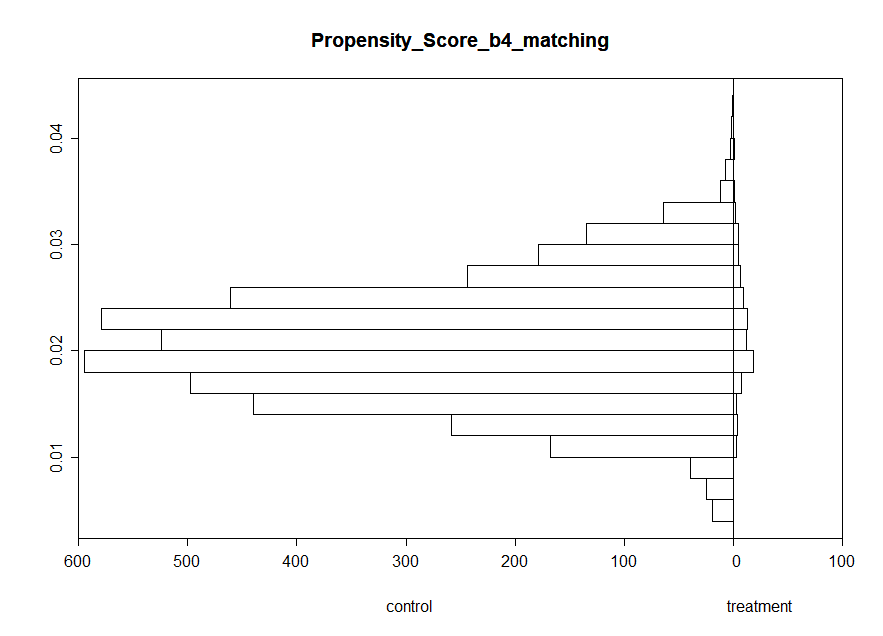
\includegraphics[width=\textwidth]{pic/b4matching.png}
	\end{figure}
\end{frame}

\begin{frame}{Propensity Score Matching}
	\begin{figure}
		\centering
		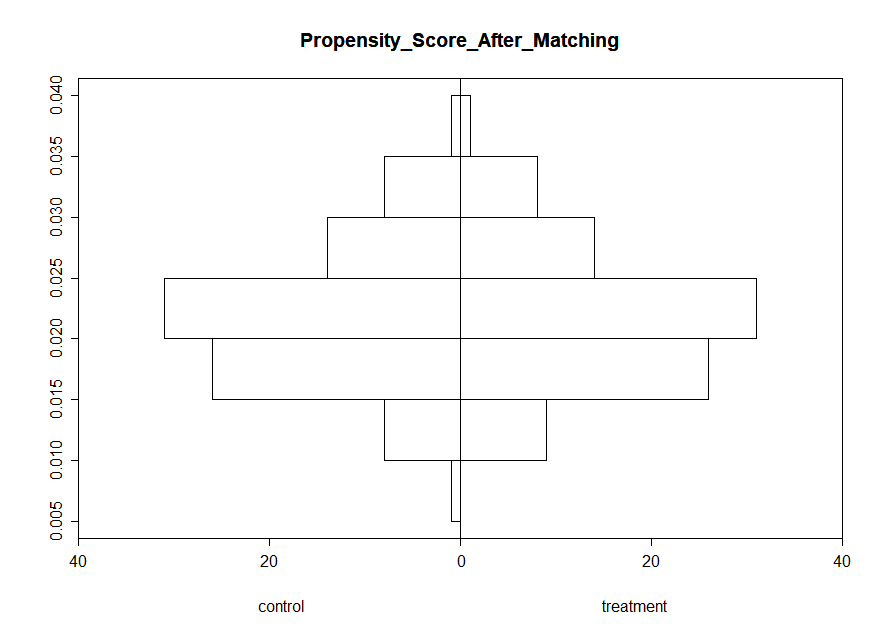
\includegraphics[width=\textwidth]{pic/Aftermatching.png}
	\end{figure}
\end{frame}

\begin{frame}{Propensity Score Matching}
	\begin{table}[!htbp] \centering 
		\caption{Results of the Online Sales and Search Effect After Nearest Propensity Score Matching: TotalMonthlySales, PagesPerDollar, and MinsPerDollar (All Product Categories)} 
		\label{tab:tablepsm} 
		\resizebox{\columnwidth}{!}{
			\begin{tabular}{@{\extracolsep{1pt}}lD{.}{.}{-3} D{.}{.}{-3} D{.}{.}{-3} D{.}{.}{-3} D{.}{.}{-3} D{.}{.}{-3} } 
				\\[-1.8ex]\hline 
				\hline \\[-1.8ex] 
				% & \multicolumn{6}{c}{\textit{Dependent variable:}} \\ 
				%\cline{2-7} 
				%\\[-1.8ex]
				& \multicolumn{2}{c}{log(TotalMonthlySales + 1)} & \multicolumn{2}{c}{log(PagesPerDollar + 1)} & \multicolumn{2}{c}{log(MinsPerDollar + 1)} \\ 
				& \multicolumn{1}{c}{Amazon-0 Mile} & \multicolumn{1}{c}{BesyBuy-0 Mile} & \multicolumn{1}{c}{Amazon-0 Mile} & \multicolumn{1}{c}{BesyBuy-0 Mile} &                             \multicolumn{1}{c}{Amazon-0 Mile} & \multicolumn{1}{c}{BesyBuy-0 Mile} \\ 
				\\[-1.8ex] & \multicolumn{1}{c}{(1)} & \multicolumn{1}{c}{(2)} & \multicolumn{1}{c}{(3)} & \multicolumn{1}{c}{(4)} & \multicolumn{1}{c}{(5)} & \multicolumn{1}{c}               {(6)}\\ 
				\hline \\[-1.8ex] 
				$\beta_1$ & 0.029 & 0.0002 & 0.00004 & 0.0001 & 0.002 & 0.00000 \\ 
				& (0.024) & (0.031) & (0.020) & (0.009) & (0.019) & (0.005) \\ 
				$\beta_2$ & -0.033 & 0.009 & -0.068^{***} & 0.003 & -0.057^{***} & 0.0004 \\ 
				& (0.028) & (0.031) & (0.023) & (0.009) & (0.022) & (0.005) \\ 
				\hline \\[-1.8ex] 
				Observations & \multicolumn{1}{c}{3,000} & \multicolumn{1}{c}{768} & \multicolumn{1}{c}{3,000} & \multicolumn{1}{c}{768} & \multicolumn{1}{c}{3,000} &                           \multicolumn{1}{c}{768} \\ 
				R$^{2}$ & \multicolumn{1}{c}{0.001} & \multicolumn{1}{c}{0.001} & \multicolumn{1}{c}{0.004} & \multicolumn{1}{c}{0.001} & \multicolumn{1}{c}{0.003} &                           \multicolumn{1}{c}{0.00004} \\ 
				Adjusted R$^{2}$ & \multicolumn{1}{c}{-0.052} & \multicolumn{1}{c}{-0.078} & \multicolumn{1}{c}{-0.048} & \multicolumn{1}{c}{-0.078} & \multicolumn{1}{c}{-0.049}               & \multicolumn{1}{c}{-0.079} \\ 
				F Statistic & \multicolumn{1}{c}{0.935 (df = 2; 2850)} & \multicolumn{1}{c}{0.192 (df = 2; 711)} & \multicolumn{1}{c}{6.219$^{***}$ (df = 2; 2850)} &                           \multicolumn{1}{c}{0.185 (df = 2; 711)} & \multicolumn{1}{c}{4.693$^{***}$ (df = 2; 2850)} & \multicolumn{1}{c}{0.014 (df = 2; 711)} \\ 
				\hline 
				\hline \\[-1.8ex] 
				\textit{Note:}  & \multicolumn{6}{r}{$^{*}$p$<$0.1; $^{**}$p$<$0.05; $^{***}$p$<$0.01} \\ 
		\end{tabular}}
	\end{table}
\end{frame}

\begin{frame}{Look-Ahead Propensity Score Matching}
	\begin{itemize}
		\item LA-PSM requires some treated observations occur over different periods $t$ and $t+k$.
		\item Basic idea in LA-PSM is to match treated observations in period $t$ with observations which were in control group in period $t$ but in treatment group in period $t+k$.
		\item In this paper, Circuit City closed all their stores at the same time: November 2008.
		\item Therefore, LA-PSM method is not applicable.
	\end{itemize}
\end{frame}

\subsection{Causal Forest}
\begin{frame}{Data Preparation for the Application}
	\begin{itemize}
		\item Our analysis is based on data individual transactions. 
		\item For each transaction $i=1,\dots,n$,
		\begin{itemize}
			\item $W_i=\texttt{CCStorePresent}_i\times\texttt{AfterStoreClosing}_i$
			\item $Y_i=\log\left(\texttt{prod\_totprice},\;\texttt{PagesPerDollar},\;\texttt{MinsPerDollar}\right)$ \footnote{right-skewed}
			\item  \textbf{10 categorical}: \texttt{hoh\_most\_education}, \texttt{census\_region}, \texttt{household\_size}, \texttt{hoh\_oldest\_age}, \texttt{children}, \texttt{racial\_background}, \texttt{connection\_speed}, \texttt{country\_of\_origin}, \texttt{prod\_category\_type} and \texttt{BBStorePresent}
			\item \textbf{4 real-valued covariates}: \texttt{pages\_viewed}\footnote{not \texttt{PagesPerDollar} is dependent variable}, \texttt{duration}\footnote{not \texttt{MinsPerDollar} is dependent variable}, \texttt{prod\_qty}, \texttt{household\_income}
			\item We expanded out categorical random variables via one-hot encoding, thus resulting in covariates $X_i \in \mathbb{R}^p$  with $p = 38$ or $p = 37$ .
		\end{itemize}
	\end{itemize}
	
\end{frame}

\begin{frame}[allowframebreaks]{The potential outcomes framework}
	For a set of i.i.d. subjects $i = 1, ..., n$, we observe a tuple $(X_i , Y_i , W_i )$, comprised of
	\begin{itemize}
		\item A \textbf{feature vector} $X_i \in \mathbb{R}^p,$
		\item A \textbf{response} $Y_i \in \mathbb{R}$, and 
		\item A \textbf{treatment assignment} $W_i \in \{0,1\}$\\~
	\end{itemize}
	
	Following the \textbf{potential outcomes} framework \citep{imbens2015causal} , we posit the existence of quantities $Y_i(0)$ and $Y_i(1)$ 
	
	\begin{itemize}
		\item These correspond to the response we would have measured given that the $i$-th subject received treatment ($W_i = 1$) or no treatment ($W_i = 0$).
	\end{itemize}
	\framebreak
	Goal is to estimate the \textbf{conditional average treatment effect}
	\begin{equation*}
		\tau(x)=\mathbb{E}\left[Y(1)-Y(0)\mid X=x\right]
	\end{equation*}
	However in experiments we only get to see $Y_i=Y_i(W_i)$
	
	\framebreak
	
	If we make no further assumptions, estimating $\tau(x)$ is not possible. 
	\begin{itemize}
		\item Literature often assumes \textbf{unconfoundedness} \citep{rosenbaum1983central}
		\begin{equation*}
			\{Y_i(0), Y_i(1)\}\perp \!\!\! \perp W_i \mid X_i.
		\end{equation*}
		\item When this assumption holds, methods based on matching or propensity score estimation are usually consistent. 
	\end{itemize}
\end{frame}

\begin{frame}{Causal Forests for Observational Studies}
	All analyses are carried out using the R package \textbf{grf}, version 1.2.0 \citep{tibshirani2018package}.
	\begin{itemize}
		\item $e(x) = \mathbb{P}[W_i\mid X_i = x]$ for the propensity score 
		\item $m(x) = \mathbb{E}[Y_i\mid X_i = x]$ for the expected outcome marginalizing over treatment
		\item An application of causal forests using \textbf{grf} \citep{athey2019estimating}: 
		\begin{enumerate}
			\item fitting two separate regression forests to estimate $m(\cdot)$ and $e(\cdot)$ (\texttt{Y.forest} and \texttt{W.forest})
			\item It then makes out-of-bag predictions using these two first-stage forests, and uses them to grow a causal forest
			\item training a pilot random forest on all the features, and then train a second forest on only those features that saw a reasonable number of splits in the first step.
		\end{enumerate}
	\end{itemize}
\end{frame}

\begin{frame}{Average Treatment Effect of Circuit City Stores Closure on amazon.com Sales}
	% The first question asks about the overall effectiveness of the intervention. 
	The package \textbf{grf} has a built-in function for average treatment effect estimation called \texttt{average\_treatment\_effect}. Using this function we obtain:
	\vspace{-1em}
	\begin{columns}
		\begin{column}{.6\textwidth}
			\begin{figure}[h]
				\centering
				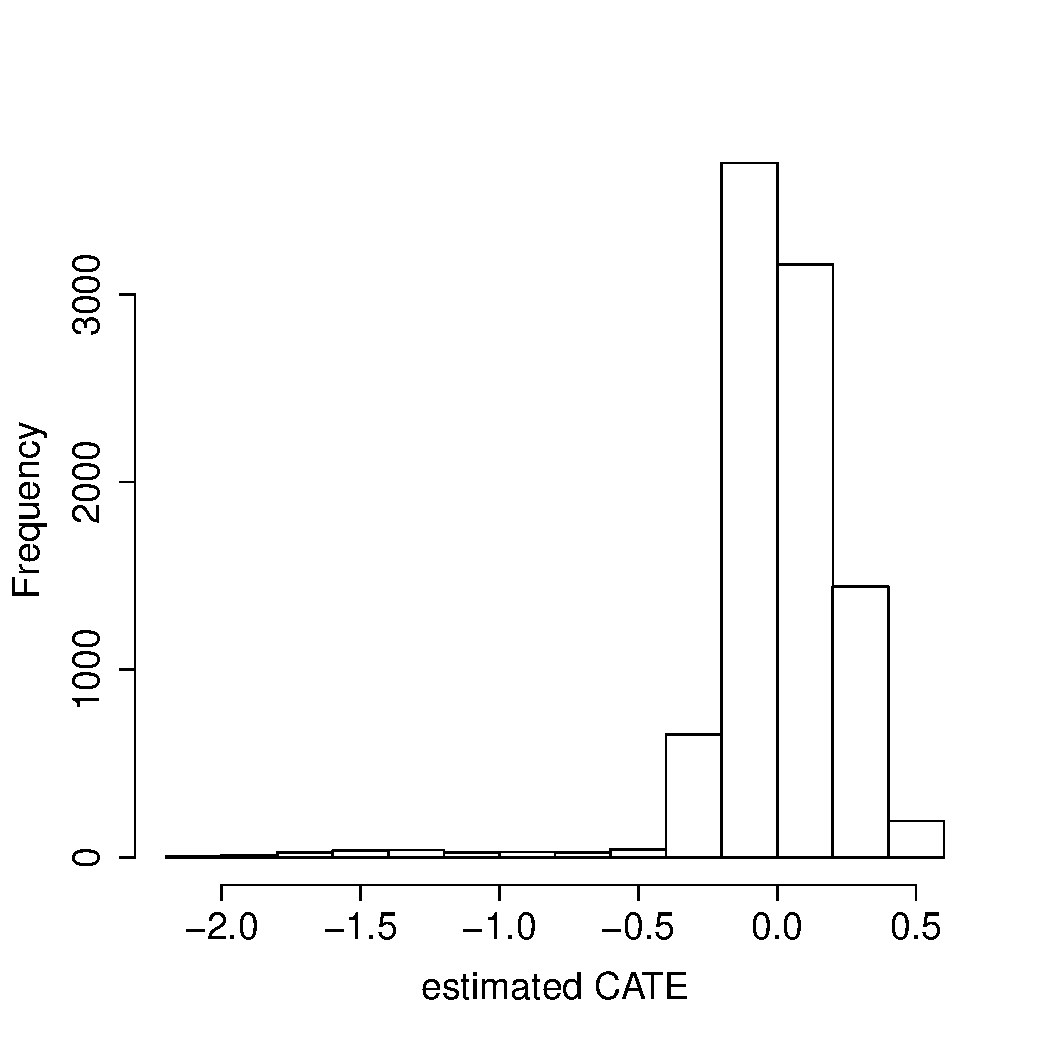
\includegraphics[scale=0.3]{pic/tauhat1_ama_hist.pdf}
				\caption{ Histogram of out-of-bag CATE estimates from a causal forest}
				\label{fig:tauhat1_ama_hist}
			\end{figure}
		\end{column}
		
		\begin{column}{.39\textwidth}
			\begin{table}[h]
				\label{}
				\caption{90\% CI for the ATT}
				\centering
				\begin{tabular}{rrr}
					\hline
					5\%  & $\hat{\tau_t}$ & 95\% \\ 
					\hline
					-0.42 & -0.22 & -0.03 \\ 
					\hline
				\end{tabular}
			\end{table}
		\end{column}
	\end{columns}
\end{frame}

\begin{frame}{Average Treatment Effect of Circuit City Stores Closure on bestbuy.com Sales}
	% The first question asks about the overall effectiveness of the intervention. 
	\vspace{-1em}
	\begin{columns}
		\begin{column}{.6\textwidth}
			\begin{figure}[h]
				\centering
				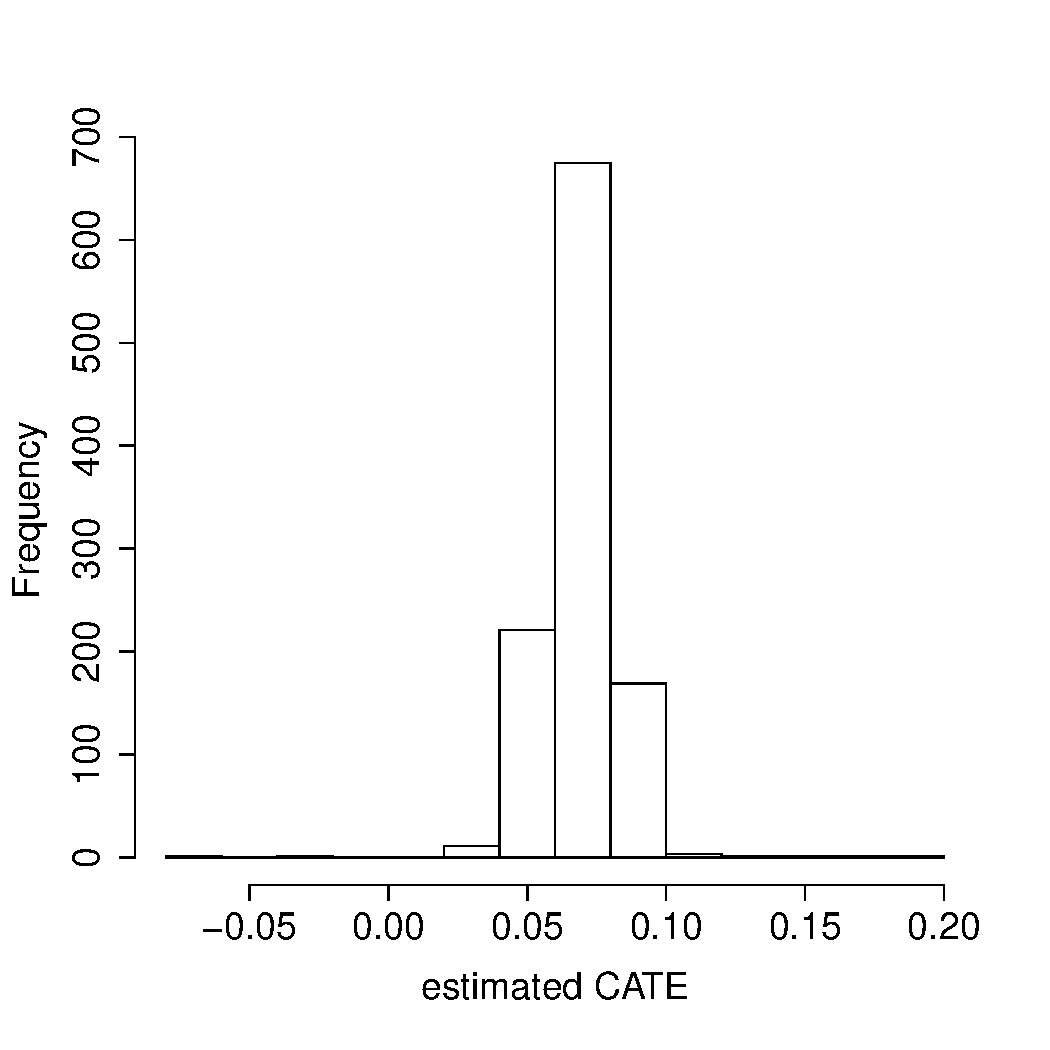
\includegraphics[scale=0.3]{pic/tauhat1_bb_hist.pdf}
				\caption{ Histogram of out-of-bag CATE estimates from a causal forest}
				\label{fig:tauhat1_bb_hist}
			\end{figure}
		\end{column}
		
		\begin{column}{.39\textwidth}
			\begin{table}[h]
				\caption{90\% CI for the ATT} 
				\centering
				\begin{tabular}{rrr}
					\hline
					5\%  & $\hat{\tau_t}$ & 95\% \\ 
					\hline
					-0.39 & 0.08 & 0.55 \\ 
					\hline
				\end{tabular}
			\end{table}
		\end{column}
	\end{columns}
\end{frame}
\begin{frame}{Average Treatment Effect of Circuit City Stores Closure on amazon.com Pages Per Dollar of Sales}
	% The first question asks about the overall effectiveness of the intervention. 
	\vspace{-1em}
	\begin{columns}
		\begin{column}{.6\textwidth}
			\begin{figure}[h]
				\centering
				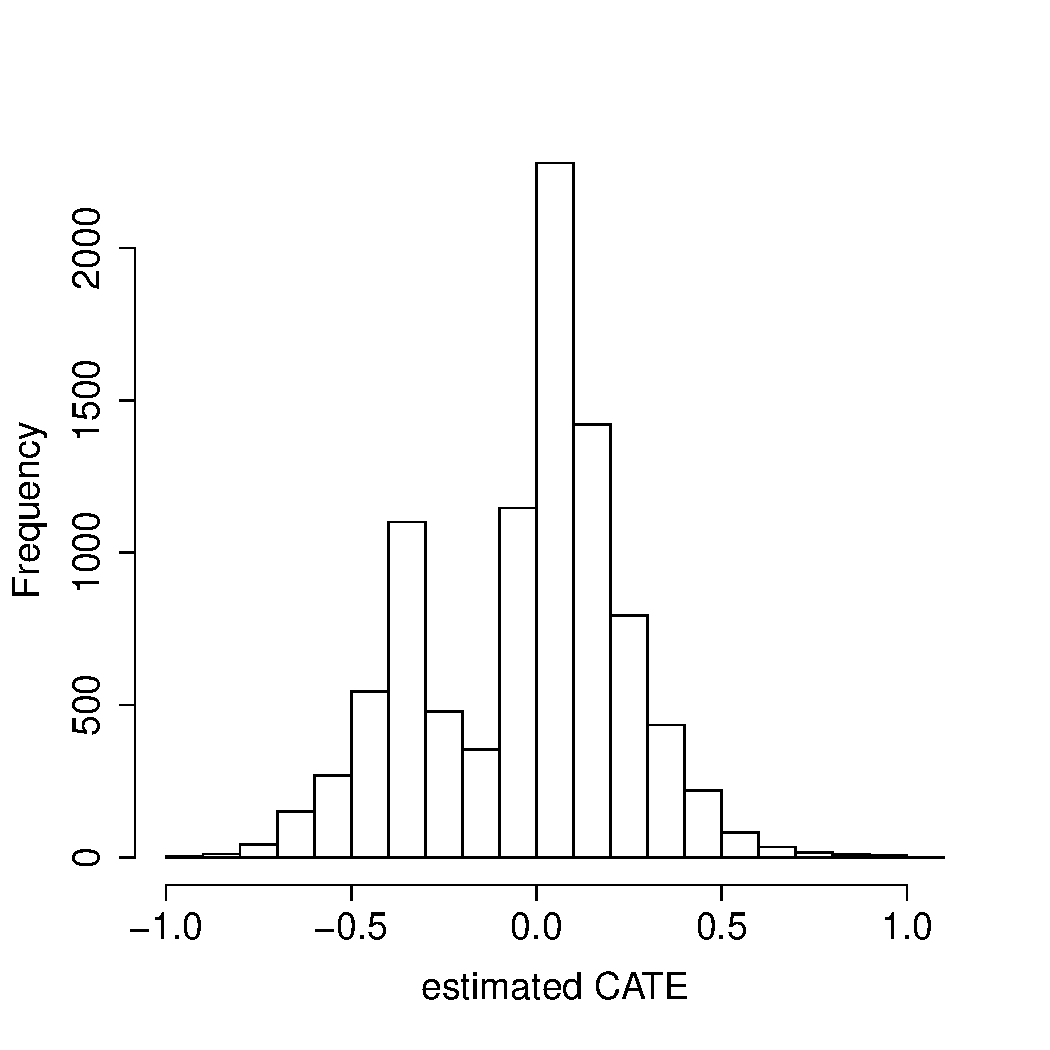
\includegraphics[scale=0.3]{pic/tauhat3_ama_hist.pdf}
				\caption{ Histogram of out-of-bag CATE estimates from a causal forest}
				\label{fig:tauhat3_ama_hist}
			\end{figure}
		\end{column}
		
		\begin{column}{.39\textwidth}
			\begin{table}[h]
				\caption{95\% CI for the ATT} 
				\centering
				\begin{tabular}{rrr}
					\hline
					2.5\%  & $\hat{\tau_t}$ & 97.5\% \\ 
					\hline
					0.02 & 0.27 & 0.52 \\ 
					\hline
				\end{tabular}
			\end{table}
		\end{column}
	\end{columns}
\end{frame}

\begin{frame}{Average Treatment Effect of Circuit City Stores Closure on bestbuy.com Pages Per Dollar of Sales}
	% The first question asks about the overall effectiveness of the intervention. 
	\vspace{-1em}
	\begin{columns}
		\begin{column}{.6\textwidth}
			\begin{figure}[h]
				\centering
				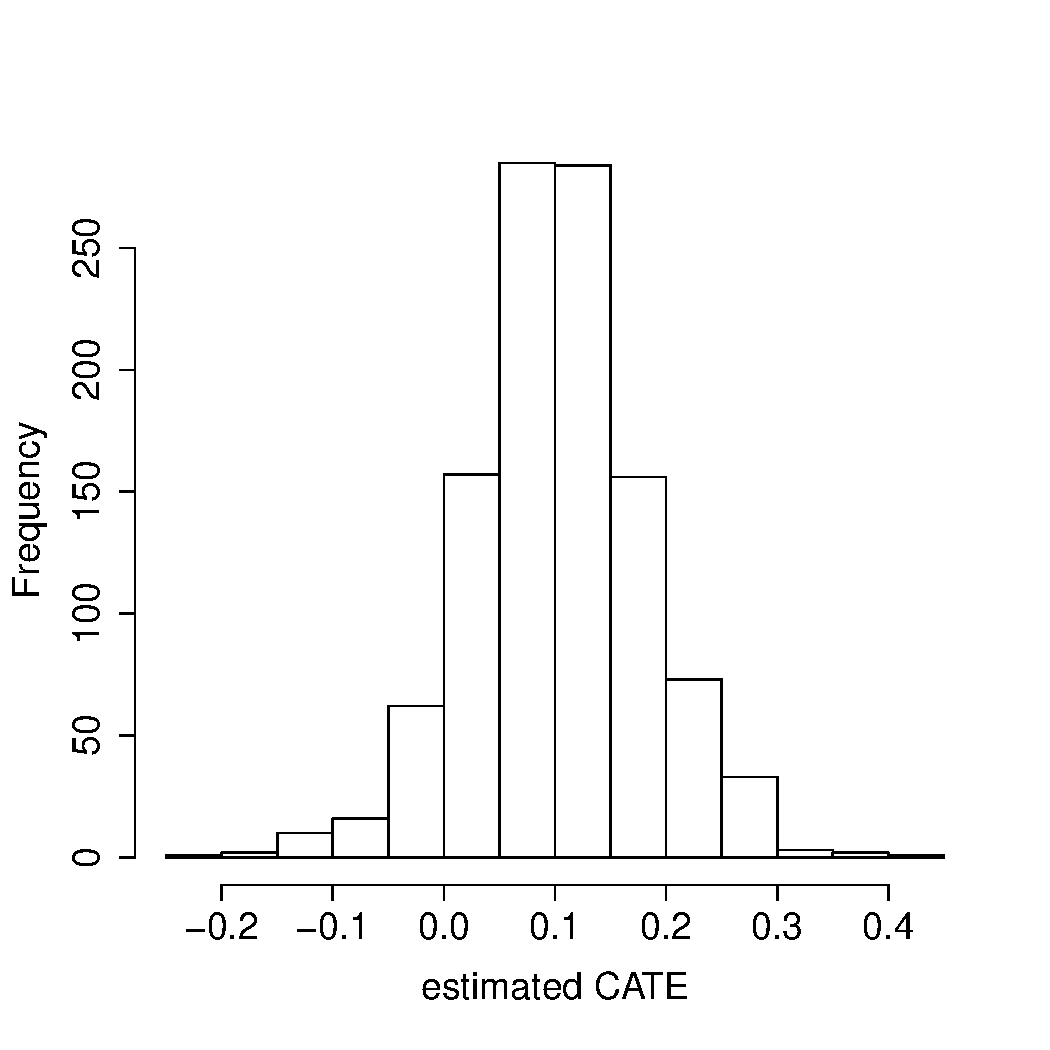
\includegraphics[scale=0.3]{pic/tauhat3_bb_hist.pdf}
				\caption{ Histogram of out-of-bag CATE estimates from a causal forest}
				\label{fig:tauhat3_bb_hist}
			\end{figure}
		\end{column}
		
		\begin{column}{.39\textwidth}
			\begin{table}[h]
				\caption{90\% CI for the ATT} 
				\centering
				\begin{tabular}{rrr}
					\hline
					5\%  & $\hat{\tau_t}$ & 95\% \\ 
					\hline
					-0.47 & 0.09 & 0.65 \\ 
					\hline
				\end{tabular}
			\end{table}
		\end{column}
	\end{columns}
\end{frame}

\begin{frame}{Average Treatment Effect of Circuit City Stores Closure on amazon.com Minutes Per Dollar of Sales}
	% The first question asks about the overall effectiveness of the intervention. 
	\vspace{-1em}
	\begin{columns}
		\begin{column}{.6\textwidth}
			\begin{figure}[h]
				\centering
				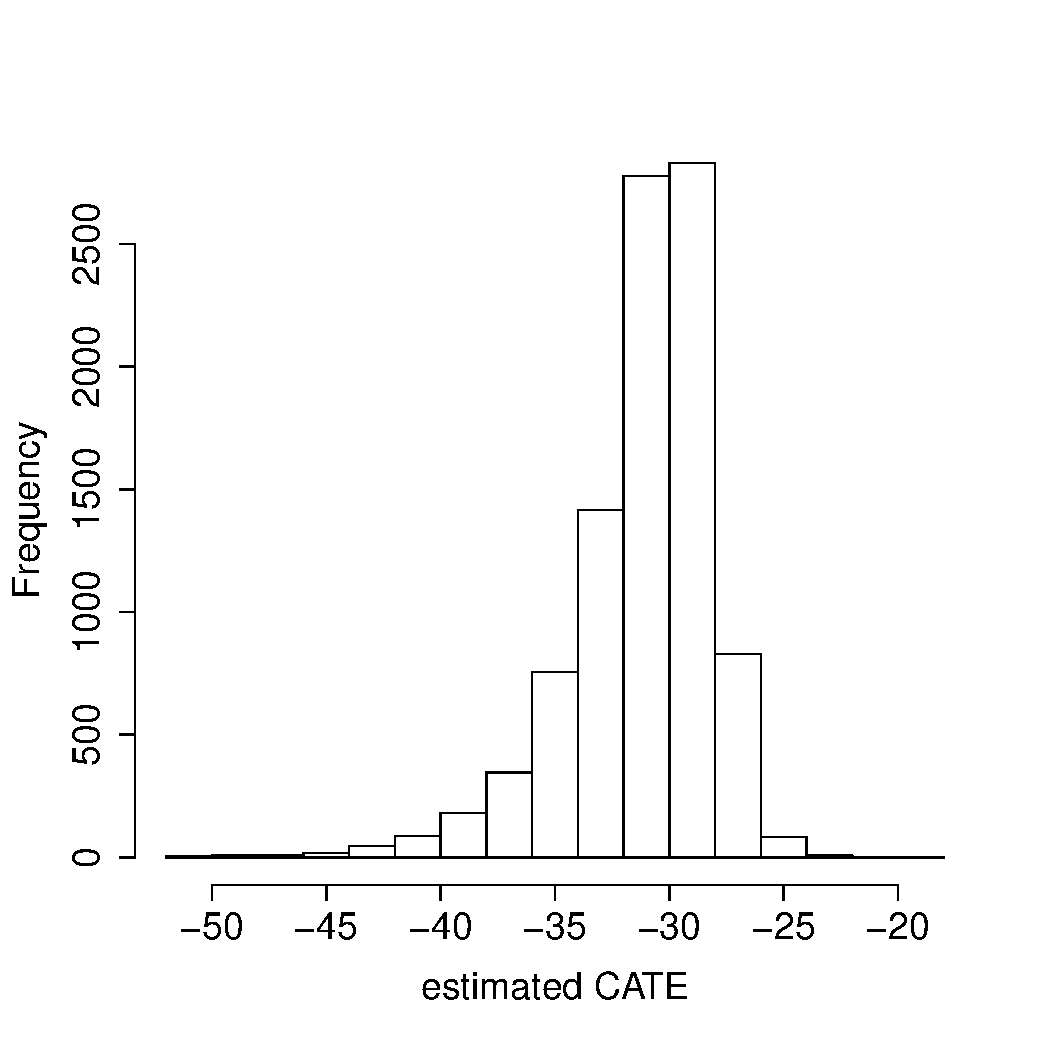
\includegraphics[scale=0.3]{pic/tauhat5_ama_hist.pdf}
				\caption{ Histogram of out-of-bag CATE estimates from a causal forest}
				\label{fig:tauhat5_ama_hist}
			\end{figure}
		\end{column}
		
		\begin{column}{.39\textwidth}
			\begin{table}[h]
				\caption{90\% CI for the ATT} 
				\centering
				\begin{tabular}{rrr}
					\hline
					5\%  & $\hat{\tau_t}$ & 95\% \\ 
					\hline
					-110.76 & -24.32 & 62.13 \\ 
					\hline
				\end{tabular}
			\end{table}
		\end{column}
	\end{columns}
\end{frame}

\begin{frame}{Average Treatment Effect of Circuit City Stores Closure on bestbuy.com Minutes Per Dollar of Sales}
	% The first question asks about the overall effectiveness of the intervention. 
	\vspace{-1em}
	\begin{columns}
		\begin{column}{.6\textwidth}
			\begin{figure}[h]
				\centering
				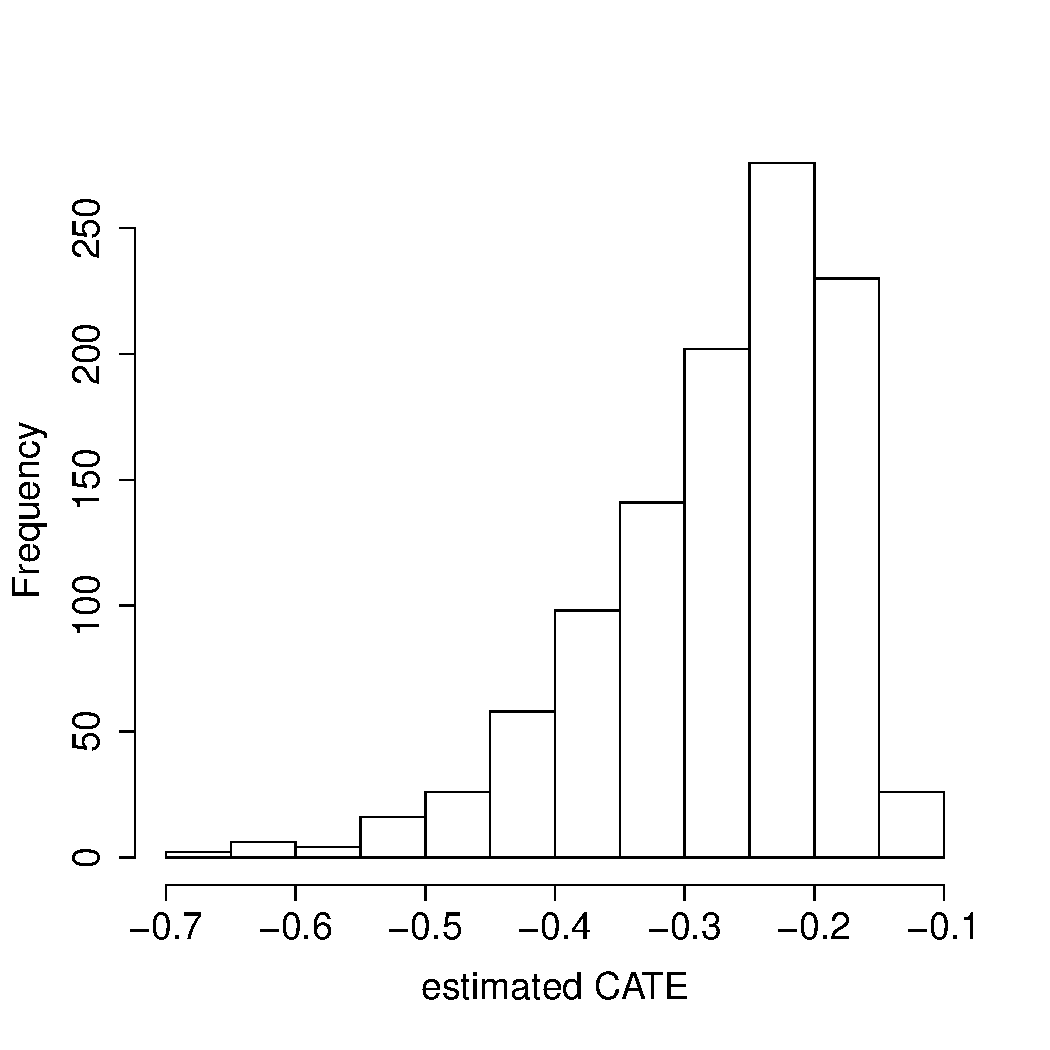
\includegraphics[scale=0.3]{pic/tauhat5_bb_hist.pdf}
				\caption{ Histogram of out-of-bag CATE estimates from a causal forest}
				\label{fig:tauhat5_bb_hist}
			\end{figure}
		\end{column}
		
		\begin{column}{.39\textwidth}
			\begin{table}[h]
				\caption{90\% CI for the ATT}
				\centering
				\begin{tabular}{rrr}
					\hline
					5\%  & $\hat{\tau_t}$ & 95\% \\ 
					\hline
					-0.63 & -0.29 & 0.05 \\ 
					\hline
				\end{tabular}
			\end{table}
		\end{column}
	\end{columns}
\end{frame}

\begin{frame}[allowframebreaks]{Reference}
	\bibliography{bobo}
	\bibliographystyle{plainnat}
\end{frame}

\end{document}


